%%%%%%%%%%%%%%%%%%%%%%%%%%%%%%%%%%%%%%%%%%%%%%%%%%%%%%%%%%%%%%%%%%%%%%%%%%%%%%%%%%%%%%%%%
%									TESIS DE DOCTORADO
%								CHRISTIAN FABIAN GARCIA ROMERO
%							   UNIVERSIDAD NACIONAL DE COLOMBIA
%
%%%%%%%%%%%%%%%%%%%%%%%%%%%%%%%%%%%%%%%%%%%%%%%%%%%%%%%%%%%%%%%%%%%%%%%%%%%%%%%%%%%%%%%%%


%%%%%%%%%%%%%%%%%%%%%%%%%%%%%%%%%%%%%%%%%%%%%%%%%%%%%%%%%%%%%%%%%%%%%%%%%%%%%%%%%%%%%%%%%

% TERCER CAPITULO: PROCESOS DE MODELAMIENTO EN ACOPLAMIENTO GEOMECÁNICO

%%%%%%%%%%%%%%%%%%%%%%%%%%%%%%%%%%%%%%%%%%%%%%%%%%%%%%%%%%%%%%%%%%%%%%%%%%%%%%%%%%%%%%%%%

%----------------------------------------------------------------------------------------
% TITULO DEL CAPITULO 3
\chapter{Modelamiento en Acoplamiento Geomecánico}~\hypertarget{chapter_03}{}
\label{ch:chapter_03}

Un problema acoplado es aquel en que dos o más modelos físicos interactúan entre sí en busca de solucionar un problema y cuyo vinculo puede ocurrir en diferentes grados de interacción\cite{Tran2005}. En un modelo geomecánico acoplado interactúan conjuntamente los modelos de flujo y geomecánico~\footnote{De ahora en adelante se entenderá como modelo \textit{geomecánico} el modelo de esfuerzos-deformación.}. Setarri \& Walters(2001) \cite{Settari2001} categorizaron diferentes tipos de acoplamiento que dependen del grado de interacción de los modelos físicos. Ese grado de interacción impacta en la exactitud de los resultados y en el costo computacional de las simulaciones. Pero esta clasificación se puede reducir a solo dos tipos de acoplamiento: (1) Modelos totalmente acoplados; (2) Modelos parcialmente acoplados.\bigskip

Los modelos totalmente acoplados combinan las ecuaciones que gobiernan los modelos de flujo y geomecánico. Las incógnitas que se resuelven en una simulación de flujo son las presiones de poros y las saturaciones de cada uno de los fluidos que conviven en el medio poroso. Las soluciones que se obtienen de una simulación geomecánica son los esfuerzos, deformaciones y desplazamientos. En un modelo totalmente acoplado se solucionan las ecuaciones diferenciales parciales de los dos modelos físicos de manera simultánea.\bigskip.

En los modelos parcialmente acoplados se hace primero la simulación de flujo, donde se obtienen los valores de presión y saturación. Esos valores entran al simulador geomecánico como parámetros iniciales y se obtiene los valores de los esfuerzos y deformaciones experimentados por el medio poroso. Luego se establece si el grado de convergencia es el deseado y de no serlo se continua con la siguiente iteración utilizando un método de convergencia como lo es el de Newton-Raphson. Cuando la convergencia es la deseada se inicia el siguiente incremento de tiempo. Esta sección se concentra en determinar los modelos totalmente acoplados que representan el problema físico acoplado. En el \textbf{Capítulo} \textbf{\ref{ch:chapter_07}} se determinaran los modelos parcialmente acoplados que harán parte del nuevo marco metodológico.\bigskip

En este capítulo se determinó los modelos que rigen el flujo en medios porosos y el comportamiento mecánico del mismo, en condiciones saturadas y parcialmente saturadas. Se encontraron expresiones matemáticas que representan estos fenómenos físicos. Con estas ecuaciones se encontraron modelos numéricos que sirvieron para crear código computacional para la simulación numérica de tres tipos de problemas comunes del acoplamiento geomecánico, todos en presencia de un medio poroso elástico e isotópico: (1) Consolidación Unidimensional; (2) Consolidación bidimensional; (3) Problema \textit{Five-Spot} en presencia de flujo bifásico~\footnote{El problema \textit{Five-Spot} es común en la ingeniería de reservorios. Ver \href{https://www.spe.org/web/csp/datasets/set02.htm}{SPE10 Benchmark} para mayor información.}.\bigskip

Con estas simulaciones se verifico que el modelo número determinado con el método de las diferencias finitas, es representativo del modelo matemático y que sirve como modelo base para las mejoras posteriores que se harán en los \textbf{Capítulos} \textbf{\ref{ch:chapter_07}} y \textbf{\ref{ch:chapter_08}}.

%----------------------------------------------------------------------------------------


%----------------------------------------------------------------------------------------
% TITULO DE LA SECCIÓN 3.1
\section{Procedimiento de modelado en Medios Porosos}~\hypertarget{sec:sec310}{}
\label{sec:sec310}

\lipsum[3-4]

\bigskip


%........................................................................................
% TITULO DE LA SUBSECCIÓN 3.1.1
\subsection{Validación en Procesos de Modelamiento}~\hypertarget{sec:sec311}{}
\label{sec:sec311}


%........................................................................................
% TITULO DE LA SUBSECCIÓN 3.1.2
\subsection{Verificación en Procesos de Modelamiento}~\hypertarget{sec:sec312}{}
\label{sec:sec312}


%........................................................................................
% TITULO DE LA SUBSECCIÓN 3.1.3
\subsection{Discrepancias en Procesos de Modelamiento}~\hypertarget{sec:sec313}{}
\label{sec:sec313}


%----------------------------------------------------------------------------------------
% TITULO DE LA SECCIÓN 3.2
\section{Modelo Conceptual}~\hypertarget{sec:sec320}{}
\label{sec:sec320}
\newpage

%----------------------------------------------------------------------------------------
% TITULO DE LA SECCIÓN 3.3
\section{Modelo Matemático}~\hypertarget{sec:sec330}{}
\label{sec:sec330}

La modelación matemática tiene como objetivo describir los diferentes aspectos del mundo real, su interacción y su dinámica a través de las matemáticas. Constituye el tercer pilar de la ciencia y la ingeniería, logrando el cumplimiento de las dos disciplinas más tradicionales, que son el análisis teórico y la experimentación \cite{Quarteroni2009MathematicalEngineering}. El modelamiento es la formulación de un modelo matemático que representa el fenómeno físico identificado en un modelo conceptual \cite{R.B.J.2013ValidationAnalysis}. Ejemplos de modelos matemáticos son el conjunto de ecuaciones diferenciales parciales que describen el equilibrio en un medio continuo, y las ecuaciones que describen el comportamiento mecánico cuando un suelo se deforma.\bigskip

Aproximadamente en la década de 1960, el análisis numérico, que es la disciplina que permite resolver ecuaciones matemáticas (algebraicas, funcionales, diferenciales e integrales) a través de algoritmos, tuvo un papel principal en la resolución de problemas vinculados al modelamiento matemático derivado de la ingeniería y las ciencias aplicadas. Después de este éxito, nuevas disciplinas comenzaron a utilizar modelos matemáticos, como la tecnología de la información y la comunicación, bioingeniería, economía, etc \cite{Quarteroni2009MathematicalEngineering}. Es por lo anterior, que se puede afirmar que el modelamiento matemático y la computación científica se están expandiendo constantemente en múltiples campos, convirtiéndose en una herramienta única para el análisis cualitativo y cuantitativo.\bigskip

En esta sección se muestra el desarrollo del modelo matemático que describe el fenómeno físico de acoplamiento geomecánico, descrito en la \textbf{Sección} \textbf{\ref{sec:sec320}}. Este modelo matemático hará referencia tanto a medios porosos saturados como parcialmente saturados. En la \textbf{Sección} \textbf{\ref{sec:sec340}} se muestra el modelo numérico derivado de este modelamiento matemático.

%........................................................................................
% TITULO DE LA SUBSECCIÓN 3.3.1
\subsection{Medio Poroso Saturado}~\hypertarget{sec:sec331}{}
\label{sec:sec331}

En estado natural un medio poroso de origen geológico, como lo son los suelos y las rocas, está constituido por tres fases: (1) Fase Solida: Minerales y/o materia orgánica; (2) Fase Liquida: Agua y/o Petróleo; (3) Fase Gaseosa: Aire o Gas Natural. Se define un medio poroso saturado, como aquel medio que tiene sus vacíos completamente saturados por un solo fluido.\bigskip

Las características del modelo geomecánico y el modelo de flujo son determinadas por esta característica del medio poroso. El flujo de líquidos en un medio poroso saturado puede ser monofásico cuando solo fluye un solo tipo de fluido, ya sea agua, petróleo o un cualquier tipo de gas. Se dice que el flujo es bifásico si fluyen dos tipos de fluidos, como es el caso de muchos de reservorios de petróleo donde fluyen al mismo tiempo petróleo y agua, cuyo mecanismo de producción es determinado por un acuífero subyacente.\bigskip

El comportamiento mecánico también es determinado por el grado de saturación del medio poroso. Para suelos saturados existen modelos constitutivos que explican su comportamiento mecánico de manera adecuada, pero que no sirven para explicar el comportamiento de suelos parcialmente saturados. En esta sección se determinará el modelo matemático geomecánico y de flujo de medios porosos saturados.\bigskip 


%........................................................................................
% TITULO DE LA SUBSECCIÓN 3.3.1.1
\subsubsection{Modelo Geomecánico}~\hypertarget{sec:sec3311}{}
\label{sec:sec3311}

El comportamiento mecánico de un medio poroso está determinado por su modelo geomecánico o también llamado modelo esfuerzo-deformación. Este modelo permite determinar: (1) Deformaciones; (2) Esfuerzos; (3) Desplazamientos. El modelo geomecánico de un medio poroso se rige por las mismas ecuaciones que definen los medios continuos, como lo son las ecuaciones de equilibrio, compatibilidad de deformaciones y el modelo constitutivo. Cuando se juntan estas tres ecuaciones se define un sistema de ecuaciones diferenciales parciales que en esencia es el modelo matemático geomecánico no-acoplado\footnote{El término "no-acoplado" se refiere a que no hay influencia del modelo de flujo en la deformación del medio.}. En la presente sección se hará una exposición simple de las ecuaciones básicas que rigen este tipo de modelo.\vspace{1cm}


\textbf{A. Ecuación de Equilibrio}
\\
La ecuación que gobierna la deformación del material sólido se llama ecuación de equilibrio. Esta se define en 2-Dimensiones como:

%----------------------------------------------------------------------------------------
% ECUACIÓN 3.1
\begin{ceqn} 
\begin{subequations} \label{eq:equ31} 
\begin{gather}
%\begin{align}
\normalsize{\frac{\partial\sigma_{xx}}{\partial x} + \frac{\partial\tau_{xy}}{\partial y} + b_x = 0} \label{eq:equ31a} \\[10pt]
\normalsize{\frac{\partial\sigma_{xx}}{\partial x} + \frac{\partial\tau_{xy}}{\partial y} + b_y = 0} \label{eq:equ31b} 
%\end{align}
\end{gather}  
\end{subequations} 
\end{ceqn}
%----------------------------------------------------------------------------------------
donde ($\sigma_{xx}$) es el esfuerzo normal horizontal, ($\sigma_{yy}$) es el esfuerzo normal vertical, ($\tau_{xy}$) es el esfuerzo cortante, ($b_{x}$) ($b_{y}$) son las componentes de las fuerzas de cuerpo del dominio del problema. Definiendo:
%----------------------------------------------------------------------------------------
% ECUACIÓN 3.2
\begin{ceqn} 
\begin{subequations} \label{eq:equ32} 
\begin{gather}
%\begin{align}
\normalsize{[\mathbf{\sigma}] = \begin{bmatrix}
       \sigma_{xx} & \tau_{xy}\\[0.3em]
       \tau_{yy} & \sigma_{yy}
       \end{bmatrix} \rightarrow 
       \{\mathbf{\sigma}\} = \begin{Bmatrix} 
       \sigma_{xx}\\[0.3em]
       \sigma_{yy}\\[0.3em]
       \tau_{xy}
       \end{Bmatrix}} \label{eq:equ32a} \\[10pt]
\normalsize{ \{\mathbf{b}\} = \begin{Bmatrix}
       b_{x} \\[0.3em]
       b_{y}
       \end{Bmatrix}} \label{eq:equ32b} \\[10pt]
\normalsize{\mathbf{S} = \begin{bmatrix}
       \frac{\partial}{\partial x} & 0\\[0.3em]
       0 & \frac{\partial}{\partial y}\\[0.3em]
       \frac{\partial}{\partial y} & \frac{\partial}{\partial x}
       \end{bmatrix}} \label{eq:equ32c} 
%\end{align}
\end{gather}  
\end{subequations} 
\end{ceqn}
%----------------------------------------------------------------------------------------

Por lo tanto la \textbf{Ecuación} \textbf{\ref{eq:equ31}} se puede escribir como:

%----------------------------------------------------------------------------------------
% ECUACIÓN 3.3
\begin{ceqn} 
\begin{gather} \label{eq:equ33} 
\normalsize{\mathbf{S}^T\{\mathbf{\sigma}\}+\{\mathbf{b}\}=\{\mathbf{0}\}}
\end{gather}  
\end{ceqn}
%----------------------------------------------------------------------------------------
donde ($\mathbf{S}$) es la matriz de deformaciones, ($\mathbf{\sigma}$) es el vector de esfuerzo total, ($\mathbf{b}$) es el vector de fuerzas de cuerpo.\vspace{1cm}


\textbf{B. Esfuerzo Efectivo}
\\
Usando la teoría de consolidación de Biot (1941)\cite{Biot1941GeneralConsolidation}, el esfuerzo total puede expresarse como la suma del esfuerzo efectivo y la presión de poros que experimenta el medio:

%----------------------------------------------------------------------------------------
% ECUACIÓN 3.4
\begin{ceqn} 
\begin{subequations} \label{eq:equ34} 
\begin{gather}
%\begin{align}
\normalsize{\sigma_{xx} = \sigma'_{xx} - \alpha p} \label{eq:equ34a} \\[6pt]
\normalsize{\sigma_{yy} = \sigma'_{yy} - \alpha p} \label{eq:equ34b} \\[6pt]
\normalsize{\tau_{xy} = \tau'_{xy} - 0 = \tau_{xy}} \label{eq:equ34c}
%\end{align}
\end{gather}  
\end{subequations} 
\end{ceqn}
%----------------------------------------------------------------------------------------
donde ($\mathbf{\sigma'_{xx}}$) es el esfuerzo efectivo horizontal,  ($\mathbf{\sigma'_{yy}}$) es el esfuerzo efectivo vertical, ($p$) es la presión de poros del medio, ($\alpha$) es el coeficiente de Biot \cite{Biot1941GeneralConsolidation}. Definiendo:

%----------------------------------------------------------------------------------------
% ECUACIÓN 3.5
\begin{ceqn} 
\begin{subequations} \label{eq:equ35} 
\begin{gather}
%\begin{align}
\normalsize{
       \{\mathbf{\sigma'}\} = \begin{Bmatrix} 
       \sigma'_{xx}\\[0.3em]
       \sigma'_{yy}\\[0.3em]
       \tau_{xy}
       \end{Bmatrix}} \label{eq:equ35a} \\[10pt]
\normalsize{ \{\mathbf{I}\} = \begin{Bmatrix}
       1 & 1 & 0
       \end{Bmatrix}} \label{eq:equ35b} \\[10pt]
\normalsize{ \alpha\{\mathbf{I}\}^T = \{\mathbf{I}\}^T - \frac{[\mathbf{D}]\{\mathbf{I}\}^T}{3K_m}} \label{eq:equ35c}
%\end{align}
\end{gather}  
\end{subequations} 
\end{ceqn}
%----------------------------------------------------------------------------------------
\\
Substituyendo las \textbf{Ecuaciones} \textbf{\ref{eq:equ32a}} y \textbf{\ref{eq:equ35}} en la \textbf{Ecuación} \textbf{\ref{eq:equ34}} se obtiene:

%----------------------------------------------------------------------------------------
% ECUACIÓN 3.6
\begin{ceqn} 
\begin{subequations} \label{eq:equ36} 
\begin{gather}
%\begin{align}
\normalsize{\{\mathbf{\sigma}\} = \{\mathbf{\sigma'}\} - \alpha\{\mathbf{I}\}^T p} \label{eq:equ36a} \\[10pt]
\normalsize{\{\mathbf{\sigma}\} = \{\mathbf{\sigma'}\} - \left(\{\mathbf{I}\}^T - \frac{[\mathbf{D}]\{\mathbf{I}\}^T}{3K_m}\right)p} \label{eq:equ36b} 
%\end{align}
\end{gather}  
\end{subequations} 
\end{ceqn}
%----------------------------------------------------------------------------------------
donde ($\mathbf{\sigma'}$) es el vector de esfuerzo efectivo, ($\mathbf{I}$) es el vector identidad, ($\mathbf{D}$) es la matriz de rigidez del modelo constitutivo.\bigskip\bigskip


\textbf{C. Relación Constitutiva}
\\
Las relaciones constitutivas se escribirán en forma general utilizando una definición incremental:
%----------------------------------------------------------------------------------------
% ECUACIÓN 3.7
\begin{ceqn} 
\begin{gather} \label{eq:equ37} 
\normalsize{d\mathbf{\sigma}'=[\mathbf{D}] d\mathbf{\epsilon}}
\end{gather}  
\end{ceqn}
%----------------------------------------------------------------------------------------
donde ($\mathbf{\epsilon}$) es el incremento de deformación total, ($\mathbf{\sigma'}$) es el incremento del esfuerzo efectivo total, ($\mathbf{D}$) es la matriz de rigidez. Definiendo:

%----------------------------------------------------------------------------------------
% ECUACIÓN 3.8
\begin{ceqn} 
\begin{gather} \label{eq:equ38} 
\normalsize{ \{\mathbf{\epsilon}\} = \begin{Bmatrix} 
       \epsilon_{xx}\\[0.3em]
       \epsilon_{yy}\\[0.3em]
       \gamma_{xy}
       \end{Bmatrix}}
\end{gather}  
\end{ceqn}
%----------------------------------------------------------------------------------------
donde ($\epsilon_{xx}$) es la deformación normal horizontal, ($\epsilon_{yy}$) es la deformación normal vertical, ($\epsilon_{xx}$) es la deformación cortante.Por lo tanto la \textbf{Ecuación} \textbf{\ref{eq:equ37}} se puede expresar:

%----------------------------------------------------------------------------------------
% ECUACIÓN 3.9
\begin{ceqn} 
\begin{gather} \label{eq:equ39} 
\normalsize{\{\mathbf{\sigma'}\}=[\mathbf{D}] \{\mathbf{\epsilon}\}}
\end{gather}  
\end{ceqn}
%----------------------------------------------------------------------------------------

La relación de compatibilidad de deformaciones se define como:

%----------------------------------------------------------------------------------------
% ECUACIÓN 3.10
\begin{ceqn} 
\begin{subequations} \label{eq:equ310} 
\begin{gather}
%\begin{align}
\normalsize{\epsilon_{xx} = \frac{\partial u_{xx}}{\partial x}} \label{eq:equ310a} \\[10pt]
\normalsize{\epsilon_{yy} = \frac{\partial v_{yy}}{\partial x} } \label{eq:equ310b} \\[10pt]
\normalsize{\gamma_{xy} = \frac{\partial v_{yy}}{\partial x} + \frac{\partial u_{xx}}{\partial y} } \label{eq:equ310c}
%\end{align}
\end{gather}  
\end{subequations} 
\end{ceqn}
%----------------------------------------------------------------------------------------
donde ($u_{xx}$) es el desplazamiento horizontal, ($u_{yy}$) es el desplazamiento vertical. Utilizando las \textbf{Ecuaciones} \textbf{\ref{eq:equ32c}} y \textbf{\ref{eq:equ38}} en la \textbf{Ecuación} \textbf{\ref{eq:equ39}} y \textbf{\ref{eq:equ310}} se obtiene:

%----------------------------------------------------------------------------------------
% ECUACIÓN 3.11
\begin{ceqn} 
\begin{subequations} \label{eq:equ311} 
\begin{gather}
%\begin{align}
\normalsize{\{\mathbf{\epsilon}\}=\mathbf{S} \{\mathbf{u}\}} \label{eq:equ311a} \\[10pt]
\normalsize{\{\mathbf{\sigma'}\}=[\mathbf{D}]\mathbf{S}\{\mathbf{u}\}} \label{eq:equ311b}
%\end{align}
\end{gather}  
\end{subequations} 
\end{ceqn}
%----------------------------------------------------------------------------------------
donde ($\mathbf{u}$) es el vector de desplazamientos.\bigskip


\textbf{D. Ecuación Geomecánica}
\\
La ecuación geomecánica es la que determina el comportamiento mecánico de un medio poroso en presencia de un cambio del esfuerzo efectivo. Para determinarla se substituye la \textbf{Ecuaciones} \textbf{\ref{eq:equ36b}} y \textbf{\ref{eq:equ311b}} en la \textbf{Ecuación} \textbf{\ref{eq:equ33}}, que resulta en:
%----------------------------------------------------------------------------------------
% ECUACIÓN 3.12

\begin{ceqn} 
\begin{subequations} \label{eq:equ312} 
\begin{gather}
%\begin{align}
\normalsize{\mathbf{S}^T\left( [\mathbf{D}]\mathbf{S}\{\mathbf{u}\} - \left(\{\mathbf{I}\}^T - \frac{[\mathbf{D}]\{\mathbf{I}\}^T}{3K_m}\right)p  \right)+\{\mathbf{b}\} = \{\mathbf{0}\}} \label{eq:equ312a} \\[10pt]
\normalsize{\mathbf{S}^T[\mathbf{D}]\mathbf{S}\{\mathbf{u}\} - \mathbf{S}^T\left(\{\mathbf{I}\}^T - \frac{[\mathbf{D}]\{\mathbf{I}\}^T}{3K_m}\right)p + \{\mathbf{b}\}=\{\mathbf{0}\}} \label{eq:equ312b}\\[10pt]
\normalsize{\mathbf{S}^T[\mathbf{D}]\mathbf{S}\{\mathbf{u}\} - \alpha\mathbf{S}^T\{\mathbf{I}\}^Tp + \{\mathbf{b}\}=\{\mathbf{0}\}} \label{eq:equ312c}
%\end{align}
\end{gather}  
\end{subequations} 
\end{ceqn}
%----------------------------------------------------------------------------------------


Reordenando simplificando se obtiene:
%----------------------------------------------------------------------------------------
% ECUACIÓN 3.13
\hfsetfillcolor{black!10}
\hfsetbordercolor{black}
\begin{ceqn} 
\begin{gather} \label{eq:equ313}
\tikzmarkin{equ313}(0.3,-0.5)(-0.3,0.6)
\normalsize{\mathbf{S}^T[\mathbf{D}]\mathbf{S}\{\mathbf{u}\} - 
\alpha\mathbf{\nabla}p  + \{\mathbf{b}\} = \{\mathbf{0}\}}
\tikzmarkend{equ313}
\end{gather}  
\end{ceqn}
%----------------------------------------------------------------------------------------

La \textbf{Ecuación} \textbf{\ref{eq:equ313}} es la relación que gobierna el comportamiento geomecánico de los medios porosos saturados. Esta ecuación tiene dos incógnitas el vector de desplazamiento y la presión de poros. Por lo tanto, otra ecuación es necesaria para resolver el problema. En la \textbf{Sección} \textbf{\ref{sec:sec3312}} se muestra la ecuación de flujo que complementa el sistema de ecuaciones.\vspace{1.0cm}


\textbf{E. Caso Elástico - Isotrópico}
\\
Un caso particular ocurre cuando el medio poroso tiene un comportamiento mecánico elástico y tiene características isotópicas. En ningún caso práctico se encuentran suelos o rocas con estas características, pero el análisis de este tipo de material permite extender después este análisis a un material con características plásticas y anisotrópicas. La matriz de rigidez para un medio poroso elástico en dos dimensiones es la siguiente:\bigskip


%----------------------------------------------------------------------------------------
% ECUACIÓN 3.14
\begin{ceqn} %\label{eq:equ314}
\begin{gather}\label{eq:equ314}
[\mathbf{D}]
=
\frac{E}{(1+\nu)(1-2\nu)}
\begin{bmatrix}
       1-\nu   & \nu     & 0 \\[0.3em]
       \nu	   & 1-\nu   & 0 \\[0.3em]
       0       & 0       &\frac{(1-2\nu)}{2}
\end{bmatrix}
\end{gather}   
\end{ceqn}
%----------------------------------------------------------------------------------------
\\
donde ($\mathbf{E}$) es el módulo de elasticidad y ($\nu$) es el módulo de Poisson. Multiplicando la \textbf{Ecuación} \textbf{\ref{eq:equ35c}} por el vector identidad ($\mathbf{I}$), y sabiendo que $\{\mathbf{I}\}\{\mathbf{I}\}^T=3$, se obtiene:

%----------------------------------------------------------------------------------------
% ECUACIÓN 3.15
\begin{ceqn} 
\begin{subequations} \label{eq:equ315} 
\begin{gather}
%\begin{align}
\alpha\{\mathbf{I}\}\{\mathbf{I}\}^T = \{\mathbf{I}\}\{\mathbf{I}\}^T - \frac{\{\mathbf{I}\}[\mathbf{D}]\{\mathbf{I}\}^T}{3\mathbf{K_m}} \label{eq:equ315a} \\[10pt]
\alpha=1-\frac{\{\mathbf{I}\}[\mathbf{D}]\{\mathbf{I}\}^T}{9K_m} \label{eq:equ315b} 
%\end{align}
\end{gather}  
\end{subequations} 
\end{ceqn}
%----------------------------------------------------------------------------------------
\bigskip

Reemplazando la \textbf{Ecuación} \textbf{\ref{eq:equ314}} en la  \textbf{Ecuación} \textbf{\ref{eq:equ315b}} se obtiene:

%----------------------------------------------------------------------------------------
% ECUACIÓN 3.16
\begin{ceqn} 
\begin{subequations} \label{eq:equ316} 
\begin{gather}
%\begin{align}
\alpha=1-\frac{1}{K_m}\frac{E}{3(1-2\nu)} \label{eq:equ316a} \\[10pt]
\alpha=1-\frac{K}{K_m} \label{eq:equ316b} 
%\end{align}
\end{gather}  
\end{subequations} 
\end{ceqn}
%----------------------------------------------------------------------------------------
donde ($K$) es el módulo de deformación volumétrica del esqueleto mineral. Sustituyendo la \textbf{Ecuación} \textbf{\ref{eq:equ314}} en la \textbf{Ecuación} \textbf{\ref{eq:equ313}} y simplificando resulta en:

%----------------------------------------------------------------------------------------
% ECUACIÓN 3.17
\begin{ceqn} %\label{eq:equ317}
\begin{gather}\label{eq:equ317}
\frac{E}{(1+\nu)(1-2\nu)}
\left[\frac{1-2\nu}{2}
\begin{bmatrix}
       \frac{\partial^2 u}{\partial x^2} + \frac{\partial^2 u}{\partial y^2}\\[1em]
       \frac{\partial^2 v}{\partial x^2} + \frac{\partial^2 v}{\partial y^2}
\end{bmatrix}
+\frac{1}{2}
\begin{bmatrix}
       \frac{\partial}{\partial x}\left(\frac{\partial u}{\partial x} + \frac{\partial v}{\partial y}\right)\\[1em]
       \frac{\partial}{\partial y}\left(\frac{\partial u}{\partial x} + \frac{\partial v}{\partial y}\right)
\end{bmatrix}
\right] - \alpha\begin{Bmatrix}  
\frac{\partial p}{ \partial x}\\[1em]
\frac{\partial p}{ \partial y}
\end{Bmatrix}
+ \begin{Bmatrix} b_{xx} \\[1em] b_{yy} \end{Bmatrix} = \begin{Bmatrix} 0 \\[1em] 0 \end{Bmatrix}
\end{gather}   
\end{ceqn}
%----------------------------------------------------------------------------------------
\\
Definiendo:

%----------------------------------------------------------------------------------------
% ECUACIÓN 3.18
\begin{ceqn} 
\begin{subequations} \label{eq:equ318} 
\begin{gather}
%\begin{align}
\normalsize{\nabla^T = \begin{Bmatrix} \frac{\partial}{\partial x} & \frac{\partial}{\partial y}\end{Bmatrix}} \label{eq:equ318a}\\[10pt]
\normalsize{\nabla \cdot \nabla = \nabla^2 = \frac{\partial^2}{\partial x^2} + \frac{\partial^2}{\partial y^2} } \label{eq:equ318b}
%\end{align}
\end{gather}  
\end{subequations} 
\end{ceqn}
%----------------------------------------------------------------------------------------
donde ($\nabla^2$) es el operador de Laplace. Simplificando la \textbf{Ecuación} \textbf{\ref{eq:equ317}} se obtiene:

%----------------------------------------------------------------------------------------
% ECUACIÓN 3.19
\begin{ceqn} %\label{eq:equ319}
\begin{gather}\label{eq:equ319}
\frac{E}{2(1+\nu)}\nabla^2 \{\mathbf{u}\}
+\frac{E}{2(1+\nu)(1-2\nu)} \nabla\left( \nabla \cdot \{\mathbf{u}\}\right)
- \alpha\nabla p + \{\mathbf{b}\} = \{\mathbf{0}\} 
\end{gather}   
\end{ceqn}
%----------------------------------------------------------------------------------------

De la teoría de la elasticidad:
%----------------------------------------------------------------------------------------
% ECUACIÓN 3.20
\begin{ceqn} %\label{eq:equ320}
\begin{gather}\label{eq:equ320}
G=\frac{E}{2(1+\nu)}
\end{gather}   
\end{ceqn}
%----------------------------------------------------------------------------------------
\\
donde ($G$) es el modulo cortante. Substituyendo las \textbf{Ecuaciones} \textbf{\ref{eq:equ320}} y \textbf{\ref{eq:equ316b}} en la \textbf{Ecuación} \textbf{\ref{eq:equ319}} resulta en:
\bigskip

%----------------------------------------------------------------------------------------
% ECUACIÓN 3.21
\hfsetfillcolor{black!10}
\hfsetbordercolor{black}
\begin{ceqn} %\label{eq:equ321}
\begin{gather}\label{eq:equ321}
%\tikzmarkin{marker-id}(below right offset)(above left offset)
\tikzmarkin{equ321}(0.5,-0.7)(-0.5,0.9)
G\nabla^2 \{\mathbf{u}\}
+\frac{G}{1-2\nu} \nabla\left( \nabla\cdot \{\mathbf{u}\}\right)
- \left[1-\frac{K}{K_m}\right]\nabla p + \{\mathbf{b}\} = \{\mathbf{0}\}
\tikzmarkend{equ321}
\end{gather}   
\end{ceqn}
%----------------------------------------------------------------------------------------
\\
La \textbf{Ecuación} \textbf{\ref{eq:equ321}} rige el comportamiento mecánico de un medio poroso isotrópico-elástico saturado. Las dos incógnitas son el campo de desplazamientos ($\mathbf{u}$) y la presión de poros del fluido que satura el medio($p$). Como se puede notar es una ecuación diferencial parcial sin términos transitorios. Al ocurrir un cambio en los esfuerzos efectivos, esta ecuación con ayuda de la ecuación de flujo determina el comportamiento acoplado del medio poroso.\bigskip



%........................................................................................
% TITULO DE LA SUBSECCIÓN 3.3.1.2
\subsubsection{Modelo de Flujo}~\hypertarget{sec:sec3312}{}
\label{sec:sec3312}


El movimiento de fluidos a través de medios porosos está gobernado por las mismas leyes fundamentales que rigen su movimiento en otros medios, como la atmósfera, redes de tuberías o fuentes de agua. Esas leyes están basadas en la conservación de la masa, momento y energía \cite{Aziz1979PetroleumSimulation}. Siguiendo el trabajo de Zienkiewicz et al.(1999) \cite{Zienkiewicz1999ComputationalGeomechanics}, se puede decir que la taza de acumulación de un fluido en un medio poroso está determinado por:

\begin{itemize}
    \item El cambio de velocidad de infiltración en el espacio.
    \item Incremento de volumen debido a un cambio en el campo de deformaciones.
    \item La compresión del fluido que satura el medio, debido a un cambio en la presión de poros.
    \item La compresión de los sólidos del medio poroso, debido a un cambio en la presión de poros.
    \item Cambio de volumen de la fase solida debido a un cambio en los esfuerzos efectivos en el contacto intergranular.
    \item Entrada o salida de fluido del volumen de control.
\end{itemize}

Lo anterior se puede escribir matemáticamente de la siguiente manera:

%----------------------------------------------------------------------------------------
% ECUACIÓN 3.22
\begin{ceqn} 
\begin{subequations} \label{eq:equ322} 
\begin{gather}
%\begin{align}
\normalsize{
\nabla^T w_{xx} + \frac{\partial \epsilon_{xx}}{\partial t} + \frac{\phi}{K_f}\frac{\partial p}{\partial t} + \frac{(1-\phi)}{K_m}\frac{\partial p}{\partial t} - \frac{K}{K_m}\left[\frac{\partial \epsilon_{xx}}{\partial t} + \frac{1}{K_m}\frac{\partial p}{\partial t}\right] + Qv_{xx}= 0
} \label{eq:equ322a}\\[10pt]
\normalsize{
\nabla^T w_{yy} + \frac{\partial \epsilon_{yy}}{\partial t} + \frac{\phi}{K_f}\frac{\partial p}{\partial t} + \frac{(1-\phi)}{K_m}\frac{\partial p}{\partial t} - \frac{K}{K_m}\left[\frac{\partial \epsilon_{yy}}{\partial t} + \frac{1}{K_m}\frac{\partial p}{\partial t}\right] + Qv_{yy}= 0
} \label{eq:equ322b}
%\end{align}
\end{gather}  
\end{subequations} 
\end{ceqn}
%----------------------------------------------------------------------------------------
\\
donde ($\mathbf{w_{xx}}$) y ($\mathbf{w_{yy}}$) son las velocidades horizontal y vertical de infiltración del fluido que satura el medio, ($K_f$) es el módulo de compresibilidad volumétrica del fluido, ($\phi$) es la porosidad del medio, ($Qv_{xx}$) y ($Qv_{yy}$) son términos fuente para incluir la entrada o salida horizontal y vertical de fluido del dominio. Definiendo:

%----------------------------------------------------------------------------------------
% ECUACIÓN 3.23
\begin{ceqn} 
\begin{subequations} \label{eq:equ323} 
\begin{gather}
%\begin{align}
\normalsize{\{\mathbf{w}\} = \begin{Bmatrix} w_{xx}\\[1em]x_{yy}\end{Bmatrix} } \label{eq:equ323a}\\[10pt]
\normalsize{\{\mathbf{Qv}\} = \begin{Bmatrix} Qv_{xx}\\[1em]Qv_{yy}\end{Bmatrix} } \label{eq:equ323b}\\[10pt]
\normalsize{K = \frac{\{\mathbf{I}\}[\mathbf{D}]\{\mathbf{I}\}^T}{9}}
%\end{align}
\end{gather}  
\end{subequations} 
\end{ceqn}
%----------------------------------------------------------------------------------------
\\
Substituyendo las \textbf{Ecuaciones} \textbf{\ref{eq:equ323}} en la \textbf{Ecuación} \textbf{\ref{eq:equ322}} y reorganizando términos, se obtiene:

%----------------------------------------------------------------------------------------
% ECUACIÓN 3.24
\begin{ceqn} %\label{eq:equ324}
\begin{gather}\label{eq:equ324}
\normalsize{\nabla^T \{\mathbf{w}\} + \left[1-\frac{\{\mathbf{I}\}[\mathbf{D}]\{\mathbf{I}\}^T}{9K_m}\right]\frac{\partial \{\mathbf{I}\}^T \{\mathbf{\epsilon}\}}{\partial t} +\left[\frac{\phi}{K_f}+\frac{(1-\phi)}{K_m}-\frac{\{\mathbf{I}\}[\mathbf{D}]\{\mathbf{I}\}^T}{(3K_{m})^{2}}\right]\frac{\partial p}{\partial t} + Qv = 0}
\end{gather}   
\end{ceqn}
%----------------------------------------------------------------------------------------
\\
donde ($\mathbf{w}$) es el vector de velocidad de infiltración, ($\mathbf{Qv}$) es el vector de términos fuente que entran y/o salen del medio. Esta ecuación es la rige el flujo en medios porosos saturados con características isotópicas y elásticas. Se tienen dos incógnitas el campo de desplazamientos y la presión de poros del fluido que satura el medio.\bigskip

La ley de Darcy\cite{Zienkiewicz1999ComputationalGeomechanics} establece que:
%----------------------------------------------------------------------------------------
% ECUACIÓN 3.25
\begin{ceqn} 
\begin{subequations} \label{eq:equ325} 
\begin{gather}
%\begin{align}
\normalsize{\{\mathbf{w}\}=-\frac{[\mathbf{K}]}{\mu}\nabla p} \label{eq:equ325a}\\[10pt]
\normalsize{[\mathbf{K}]=\begin{bmatrix} 
k_{xx} & k_{xy}\\[1em]
k_{xy} & k_{yy}
\end{bmatrix} } \label{eq:equ325b}
%\end{align}
\end{gather}  
\end{subequations} 
\end{ceqn}
%----------------------------------------------------------------------------------------
donde ($\mathbf{K}$) es el tensor de permeabilidad, ($\mu$) es la viscosidad dinámica del fluido que satura el medio. Reemplazando las \textbf{Ecuaciones} \textbf{\ref{eq:equ325}} y \textbf{\ref{eq:equ311a}} en la \textbf{Ecuación} \textbf{\ref{eq:equ324}} se obtiene:

%----------------------------------------------------------------------------------------
% ECUACIÓN 3.26
\hfsetfillcolor{black!10}
\hfsetbordercolor{black}
\begin{ceqn} %\label{eq:equ326}
\begin{gather}\label{eq:equ326}
\tikzmarkin{equ326}(0.5,-0.7)(-0.5,0.9)
\normalsize{\nabla^T \left[\frac{[\mathbf{K}]}{\mu}\nabla p\right] = \alpha\frac{\partial \nabla^T \{\mathbf{u}\}}{\partial t} +\left[\frac{\phi}{K_f}+\frac{(1-\phi)}{K_m}-\frac{\{\mathbf{I}\}[\mathbf{D}]\{\mathbf{I}\}^T}{(3K_{m})^{2}}\right]\frac{\partial p}{\partial t} + Qv}
\tikzmarkend{equ326}
\end{gather}   
\end{ceqn}
%----------------------------------------------------------------------------------------
\\
La \textbf{Ecuación} \textbf{\ref{eq:equ326}} rige el flujo en un medio poroso saturado. Esta ecuación rige el comportamiento de medios porosos tanto elásticos como elastoplásticos. En conjunto con la \textbf{Ecuación} \textbf{\ref{eq:equ313}} se tiene el sistema de ecuaciones del modelo geomecánico acoplado. Como se verá en el \textbf{Capítulo}  \textbf{\ref{ch:chapter_07}} este modelo acoplado se podrá resolver de manera totalmente acoplada o por medio de un acoplamiento iterativo.\vspace{0.4cm}


%........................................................................................
% TITULO DE LA SUBSECCIÓN 3.3.2
\subsection{Medio Poroso Parcialmente Saturado}~\hypertarget{sec:sec332}{}
\label{sec:sec332}

Un medio poroso parcialmente saturado tiene en sus vacíos dos o más fluidos que saturan el medio. Por ejemplo, un suelo residual que se caracteriza por estar parcialmente saturado, en sus vacíos tiene agua y aire. Un reservorio de petróleo se caracteriza porque en los vacíos de la roca que conforma el reservorio puede existir hasta tres tipos de fluido: Gas, petróleo y agua.\bigskip

En esta sección se tomarán las \textbf{Ecuaciones} \textbf{\ref{eq:equ313}} y \textbf{\ref{eq:equ326}} como base para determinar el modelo matemático de un medio poroso parcialmente saturado. En esta investigación se tiene como alcance el estudio de medios porosos en presencia de flujo bifásico. Por lo tanto, el modelo será función de un fluido que moje preferencialmente el medio poroso, que se conoce como fluido mojado, y un fluido no-mojado.\bigskip

%////////////////////////////////////////////////////////////////////////////////////////
% Figura 3.1
\begin{figure}[!ht]
\centering
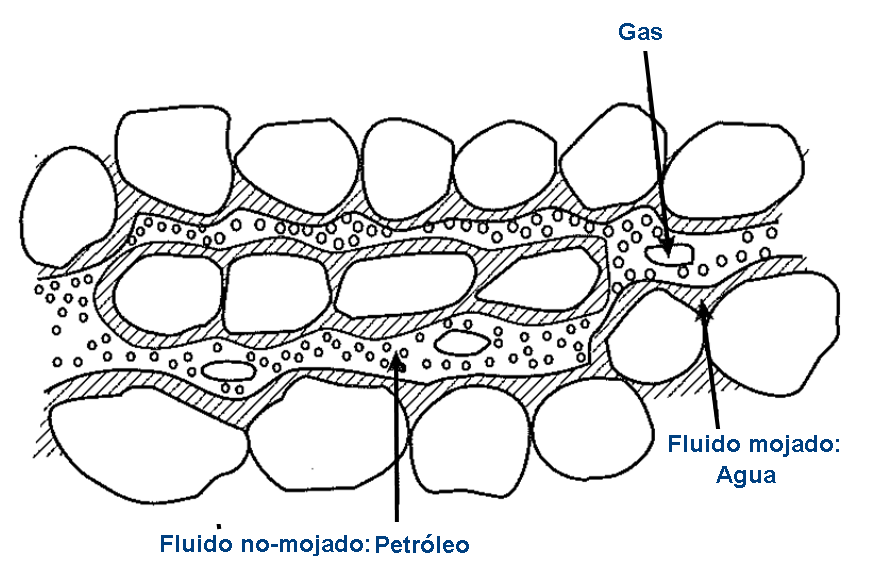
\includegraphics[width=7cm]{Imagenes/Mojabilidad.png}
\caption[Distribución de los fluidos mojado y no-mojado]{Distribución de los fluidos mojado y no-mojado. Modificado de Rosa et al.(2006) \cite{Rosa2006EngenhariaPetroleo}}
\label{fig:fig31}
\end{figure}
%/////////////////////////////////////////////////////////////////////////////////////////

En un reservorio de petróleo se sabe que el agua moja preferencialmente la roca en la mayoría de los casos, como se ve en la \textbf{Figura} \ref{fig:fig31}. El gas se mantiene en los canales centrales de los poros puesto que es un fluido que presenta la menor tendencia de mojar preferencialmente la roca. El agua estaría en las paredes de los poros junto a las partículas sólidas de la roca. El petróleo por ser un fluido intermediario en términos de mojabilidad, estaría localizado entre el agua y el gas.\bigskip

En un suelo parcialmente saturado, es el agua quien moja preferencialmente los sólidos del suelo, y por eso se le denomina al agua como el fluido mojado. El aire en los vacíos del suelo presenta una menor tendencia de mojar los sólidos del suelo y por eso se le considera como el fluido no-mojado.\bigskip

%........................................................................................
% TITULO DE LA SUBSECCIÓN 3.3.2.1
\subsubsection{Modelo Geomecánico}~\hypertarget{sec:sec3321}{}
\label{sec:sec3321}

Para empezar la determinación del modelo geomecánico de un medio poroso parcialmente saturado, se deben hacer primero unas definiciones.\bigskip\bigskip

\textbf{A. Saturación}
\\
El grado de saturación ($S$) se define como la razón entre el volumen de vacíos y el volumen total del medio poroso. Para un suelo saturado, el grado de saturación del fluido es 100\%. Para un medio parcialmente saturado, el grado de saturación es la suma de la saturación del fluido mojado más la saturación del fluido no-mojado, como se muestra en la siguiente ecuación:\bigskip

%----------------------------------------------------------------------------------------
% ECUACIÓN 3.27
\begin{ceqn} 
\begin{gather} \label{eq:equ27} 
S_w + S_n = 1
\end{gather}  
\end{ceqn}
%----------------------------------------------------------------------------------------
\\
donde ($S_w$) es la saturación del fluido mojado y ($S_n$) es la saturación del fluido no-mojado.\bigskip\bigskip


\textbf{B. Presión Capilar}
\\
Cuando se habla de flujo bifásico se debe tener en cuenta la presión capilar ($P_c$). La presión capilar es la diferencia de presión a través de la interfase que separa dos fluidos inmiscibles, cuando se ponen en contacto en un medio poroso. Con ayuda de la presión capilar se establece la relación que existe entre el fluido mojado y el fluido no-mojado, como se como se muestra en la siguiente ecuación:\bigskip

%----------------------------------------------------------------------------------------
% ECUACIÓN 3.28
\begin{ceqn} 
\begin{gather} \label{eq:equ328} 
P_c = p_n - p_w
\end{gather}  
\end{ceqn}
%----------------------------------------------------------------------------------------
\\
donde ($p_n$) es la presión de poros del fluido no-mojado y ($p_w$) es la presión de poros del fluido mojado.\bigskip\bigskip


\textbf{C. Tasa de Saturación}
\\
En flujo bifásico es importante determinar cuál es la tasa de cambio de la saturación de los fluidos mojado y no-mojado, referente al tiempo. Con ayuda de la regla de la cadena se puede escribir:

%----------------------------------------------------------------------------------------
% ECUACIÓN 3.29
\begin{ceqn} 
\begin{subequations} \label{eq:equ329} 
%\begin{gather}
\begin{align}
\shortintertext{Fluido mojado:} &\frac{\partial S_w}{\partial t} = \frac{\partial S_w}{\partial P_c}\frac{\partial P_c}{\partial t} \label{eq:equ329a} \\[10pt]
\shortintertext{Fluido no-mojado:} 			&\frac{\partial S_n}{\partial t} = \frac{\partial S_n}{\partial P_c}\frac{\partial P_c}{\partial t} \label{eq:equ329b}
\end{align}
%\end{gather}  
\end{subequations} 
\end{ceqn}
%----------------------------------------------------------------------------------------
\\
Remplazando la \textbf{Ecuación} \textbf{\ref{eq:equ328}} en la \textbf{Ecuación} \textbf{\ref{eq:equ329}} se obtiene:

%----------------------------------------------------------------------------------------
% ECUACIÓN 3.30
\begin{ceqn} 
\begin{subequations} \label{eq:equ330} 
%\begin{gather}
\begin{align}
\shortintertext{Fluido mojado:}     &\frac{\partial S_w}{\partial t} = \frac{\partial S_w}{\partial P_c}\left[\frac{\partial p_n}{\partial t}-\frac{\partial p_w}{\partial t}\right] = S'_w\left[\frac{\partial p_n}{\partial t}-\frac{\partial p_w}{\partial t}\right] \label{eq:equ330a} \\[10pt]
\shortintertext{Fluido no-mojado:} 	&\frac{\partial S_n}{\partial t} = \frac{\partial S_n}{\partial P_c}\left[\frac{\partial p_w}{\partial t}-\frac{\partial p_w}{\partial t}\right] = -S'_w\left[\frac{\partial p_w}{\partial t}-\frac{\partial p_w}{\partial t}\right] \label{eq:equ330b}
\end{align}
%\end{gather}  
\end{subequations} 
\end{ceqn}
%----------------------------------------------------------------------------------------
\\
\textbf{D. Presión de Poros Promedio}
\\
En presencia de flujo bifásico se puede determinar la presión promedio de poros como la suma de las contribuciones de presión de poros de cada fluido, ponderadas con sus respectivas saturaciones, como se ve en la siguiente ecuación:

%----------------------------------------------------------------------------------------
% ECUACIÓN 3.31
\begin{ceqn} 
\begin{gather} \label{eq:equ331} 
\overline{p} = S_w p_w + S_n p_n
\end{gather}  
\end{ceqn}
%----------------------------------------------------------------------------------------
\\
\textbf{E. Tasa de Presión de Poros Promedio}
\\
Como se puede ver en la \textbf{Ecuación} \textbf{\ref{eq:equ326}} es necesario determinar la tasa de variación de la presión de poros. Para tener en cuenta las presiones de poros de los fluidos mojado y no-mojado es necesario derivar la \textbf{Ecuación} \textbf{\ref{eq:equ331}} con respecto al tiempo. Con ayuda de la regla de la cadena se obtiene:\bigskip

%----------------------------------------------------------------------------------------
% ECUACIÓN 3.32
\begin{ceqn} 
\begin{gather} \label{eq:equ332} 
\frac{\partial \overline{p}}{\partial t} = p_w\frac{\partial S_w}{\partial t} + S_w\frac{\partial p_w}{\partial t} + p_n\frac{\partial S_n}{\partial t} + p_n\frac{\partial S_n}{\partial t}
\end{gather}  
\end{ceqn}
%----------------------------------------------------------------------------------------
\\
Substituyendo la \textbf{Ecuación} \textbf{\ref{eq:equ330}} en la \textbf{Ecuación} \textbf{\ref{eq:equ332}} se obtiene:

%----------------------------------------------------------------------------------------
% ECUACIÓN 3.33
\begin{ceqn} 
\begin{subequations} \label{eq:equ333} 
\begin{gather}
%\begin{align}
\frac{\partial \overline{p}}{\partial t} = p_w S'_w\left[\frac{\partial p_n}{\partial t}-\frac{\partial p_w}{\partial t}\right] + S_w\frac{\partial p_w}{\partial t} - p_n S'_w\left[\frac{\partial p_n}{\partial t}-\frac{\partial p_w}{\partial t}\right] + p_n\frac{\partial S_n}{\partial t} \label{eq:equ333a} \\[12pt]
\frac{\partial \overline{p}}{\partial t} = \left[S_w + P_c S'_w\right]\frac{\partial p_w}{\partial t} + \left[S_n - P_c S'_w\right]\frac{\partial p_n}{\partial t}  \label{eq:equ333b} \\[12pt]
\frac{\partial \overline{p}}{\partial t} = S''_w\frac{\partial p_w}{\partial t} + S''_n\frac{\partial p_n}{\partial t}  \label{eq:equ333c}
%\end{align}
\end{gather}  
\end{subequations} 
\end{ceqn}
%----------------------------------------------------------------------------------------
%\bigskip\bigskip

\textbf{F. Gradiente de la Presión de Poros Promedio}
\\
De la misma forma como se determino la \textbf{Ecuación} \textbf{\ref{eq:equ333c}}, se puede obtener la variación de la presión de poros promedio respecto al espacio:

%----------------------------------------------------------------------------------------
% ECUACIÓN 3.34
\begin{ceqn} 
\begin{gather} \label{eq:equ334} 
\nabla \overline{p} = S''_w\nabla p_w + S''_n\nabla p_n
\end{gather}  
\end{ceqn}
%----------------------------------------------------------------------------------------
\bigskip

\textbf{G. Modelo Geomecánico Medio Poroso Parcialmente Saturado}
\\
Finalmente se puede obtener el modelo geomecánico para un medio poroso parcialmente saturado. Se substituye la \textbf{Ecuación} \textbf{\ref{eq:equ334}} en la \textbf{Ecuación} \textbf{\ref{eq:equ313}} y se obtiene:\bigskip

%----------------------------------------------------------------------------------------
% ECUACIÓN 3.35

\begin{ceqn} 
\begin{subequations} \label{eq:equ335} 
\begin{gather}
%\begin{align}
\tikzmarkin{equ335}(0.5,-0.5)(-0.5,0.7)
\normalsize{\mathbf{S}^T[\mathbf{D}]\mathbf{S}\{\mathbf{u}\} - 
\alpha S''_w\nabla p_w + \alpha S''_n\nabla p_n + \{\mathbf{b}\} = \{\mathbf{0}\}}
\tikzmarkend{equ335}\label{eq:equ335a} \\[12pt]
S''_w = S_w + P_c\frac{\partial S_w}{\partial P_c}  \label{eq:equ335b} \\[12pt]
S''_n = S_n - P_c\frac{\partial S_n}{\partial P_c}  \label{eq:equ335c} \\[12pt]
P_c = \mathnormal{f}(S_w) = p_n - p_w  \label{eq:equ335d}
%\end{align}
\end{gather}
\end{subequations} 
\end{ceqn}
%----------------------------------------------------------------------------------------
\\
Esta ecuación gobierna el comportamiento mecánico de medios poroso parcialmente saturados cuando están en presencia de flujo bifásico. La incógnita de esta ecuación sigue siendo el campo de desplazamientos, pero se suma ahora la presión de poros del fluido mojado ($p_w$), la presión de poros del fluido no-mojado ($p_n$), la saturación del fluido mojado ($S_w$) y la saturación del fluido no-mojado ($S_n$).\bigskip\bigskip 

\textbf{H. Modelo Geomecánico Medio Poroso Parcialmente Saturado - Caso Elástico}
\\
Para el caso especial que el medio poroso sea elástico e isotrópico la \textbf{Ecuación} \textbf{\ref{eq:equ335}} se puede escribir de la siguiente forma:


%----------------------------------------------------------------------------------------
% ECUACIÓN 3.36
\hfsetfillcolor{black!10}
\hfsetbordercolor{black}
\begin{ceqn} 
\begin{subequations} \label{eq:equ336} 
\begin{gather}
%\begin{align}
\tikzmarkin{equ336}(0.25,-0.7)(-0.25,0.9)
\normalsize{G\nabla^2 \{\mathbf{u}\}
+\frac{G}{1-2\nu} \nabla\left( \nabla\cdot \{\mathbf{u}\}\right)
- \left[1-\frac{K}{K_m}\right]S''_w\nabla p_w - \left[1-\frac{K}{K_m}\right]S''_n\nabla p_n + \{\mathbf{b}\} = \{\mathbf{0}\}}
\tikzmarkend{equ336}\label{eq:equ336a} \\[12pt]
S''_w = S_w + P_c\frac{\partial S_w}{\partial P_c}  \label{eq:equ336b} \\[12pt]
S''_n = S_n - P_c\frac{\partial S_n}{\partial P_c}  \label{eq:equ336c} \\[12pt]
P_c = \mathnormal{f}(S_w) = p_n - p_w  \label{eq:equ336d} \\[12pt]
\alpha=1-\frac{K}{K_m}  \label{eq:equ336e}
%\end{align}
\end{gather}  
\end{subequations} 
\end{ceqn}
%----------------------------------------------------------------------------------------


%........................................................................................
% TITULO DE LA SUBSECCIÓN 3.3.2.2
\subsubsection{Modelo de Flujo}~\hypertarget{sec:sec3322}{}
\label{sec:sec3322}

Para obtener el modelo de flujo bifásico se utilizara la misma metodología usada por Zienkiewicz et al.(1999) \cite{Zienkiewicz1999ComputationalGeomechanics}, para determinar la tasa de acumulación de fluidos en un medio poroso, como ya se mostró en la determinación de la \textbf{Ecuación} \textbf{\ref{eq:equ322}}. Para un medio poroso parcialmente saturado la tasa de acumulación de fluido mojado se puede expresar de la siguiente forma:
\bigskip
%----------------------------------------------------------------------------------------
% ECUACIÓN 3.37
\begin{ceqn} %\label{eq:equ337}
\begin{gather}\label{eq:equ337}
\nabla^T \{\mathbf{w}\} + S_w \frac{\alpha - \phi}{K_m}\frac{\partial \overline{p}}{\partial t} + \phi\frac{\partial S_w}{\partial t} + \alpha S_w\frac{\partial\mathbf{I}^T \{\mathbf{\epsilon}\}}{\partial t} + S_w\frac{\phi}{K_w}\frac{\partial p_w}{\partial t} + Q_w= 0
\end{gather}   
\end{ceqn}
%----------------------------------------------------------------------------------------
\bigskip

Substituyendo las \textbf{Ecuaciones} \textbf{\ref{eq:equ334}}, \textbf{\ref{eq:equ325a}} y \textbf{\ref{eq:equ330a}} en la \textbf{Ecuación} \textbf{\ref{eq:equ337}} resulta en:\bigskip

%----------------------------------------------------------------------------------------
% ECUACIÓN 3.38
\begin{ceqn}
\begin{align}\label{eq:equ338}
 \nabla^T \left[\frac{k k_{rw}}{\mu_{w}}\nabla p_w\right] &= S_w \frac{\alpha - \phi}{K_m}\left[S''_w\frac{\partial p_w}{\partial t} + S''_n\frac{\partial p_n}{\partial t}\right] + \phi\frac{\partial S_w}{\partial P_c}\left[\frac{\partial p_n}{\partial t} - \frac{\partial p_w}{\partial t} \right] \nonumber \\[12pt]
  &\qquad {} + \alpha S_w\frac{\partial \mathbf{I}^T \{\mathbf{\epsilon}\}}{\partial t} +S_w\frac{\phi}{K_w}\frac{\partial p_w}{\partial t} + Q_w
\end{align}
\end{ceqn}
%----------------------------------------------------------------------------------------
\bigskip

Simplificando y reordenando, se obtiene la ecuación de flujo para el fluido mojado:
%----------------------------------------------------------------------------------------
% ECUACIÓN 3.39
\hfsetfillcolor{black!10}
\hfsetbordercolor{black}
\begin{ceqn} 
\begin{subequations} \label{eq:equ339} 
\begin{gather}
\begin{multlined}
\tikzmarkin{equ339}(0.25,-0.5)(-0.25,0.7)
\nabla^T \left[\frac{k k_{rw}}{\mu_{w}}\nabla p_w\right] = \left[S_w \frac{\alpha - \phi}{K_m}S''_w + \phi\frac{S_w}{K_w} - \phi\frac{\partial S_w}{\partial P_c}\right]\frac{\partial p_w}{\partial t} \\[10pt]
+ \left[S_w \frac{\alpha - \phi}{K_m}S''_n + \phi\frac{\partial S_w}{\partial P_c}\right]\frac{\partial p_n}{\partial t} +\alpha S_w\frac{\partial \nabla^T \{\mathbf{u}\}}{\partial t} + Q_w \tikzmarkend{equ339} \label{eq:equ339a}
\end{multlined}\\[12pt]
S''_w = S_w + P_c\frac{\partial S_w}{\partial P_c}  \label{eq:equ339b}\\[12pt]
S''_n = S_n - P_c\frac{\partial S_w}{\partial P_c}  \label{eq:equ339c}
\end{gather}  
\end{subequations} 
\end{ceqn}
%----------------------------------------------------------------------------------------
\bigskip

Con el mismo procedimiento se obtiene la ecuación de flujo para el fluido no-mojado:
%----------------------------------------------------------------------------------------
% ECUACIÓN 3.40
\hfsetfillcolor{black!10}
\hfsetbordercolor{black}
\begin{ceqn} 
\begin{subequations} \label{eq:equ340} 
\begin{gather}
\begin{multlined}
\tikzmarkin{equ340}(0.25,-0.5)(-0.25,0.7)
\nabla^T \left[\frac{k k_{rn}}{\mu_{n}}\nabla p_n\right] = \left[S_n \frac{\alpha - \phi}{K_m}S''_n + \phi\frac{S_n}{K_n} - \phi\frac{\partial S_w}{\partial P_c}\right]\frac{\partial p_n}{\partial t} \\[10pt]
+ \left[S_n \frac{\alpha - \phi}{K_m}S''_w + \phi\frac{\partial S_w}{\partial P_c}\right]\frac{\partial p_w}{\partial t} +\alpha S_n\frac{\partial \nabla^T \{\mathbf{u}\}}{\partial t} + Q_n \tikzmarkend{equ340} \label{eq:equ340a}
\end{multlined}\\[12pt]
S''_w = S_w + P_c\frac{\partial S_w}{\partial P_c}  \label{eq:equ340b}\\[12pt]
S''_n = S_n - P_c\frac{\partial S_w}{\partial P_c}  \label{eq:equ340c}
\end{gather}  
\end{subequations} 
\end{ceqn}
%----------------------------------------------------------------------------------------



%----------------------------------------------------------------------------------------
% TITULO DE LA SECCIÓN 3.4
\section{Modelo Numérico}~\hypertarget{sec:sec340}{}
\label{sec:sec340}

En la actualidad, el modelamiento numérico se usa ampliamente para simular el comportamiento de suelos y rocas en varios proyectos geotécnicos. Los métodos numéricos utilizados en el modelamiento de estos geomateriales incluyen el método de elementos finitos (MEF), el método de elementos de contorno (MEC), el método de diferencias finitas (MDF) y el método de elementos discretos (MED) \cite{Li2018RockboltingApplications}.\bigskip 

Cualquiera que sea el método que se escoja para la simulación numérica del problema geotécnico que se desee resolver, es necesario partir de formulaciones matemáticas, como las de la sección anterior, y discretizar tanto en el dominio del espacio como en el dominio del tiempo\footnote{En el dominio del tiempo para problemas transitorios, como el flujo en medios porosos}.\bigskip

En esta sección se utilizará el método de los elementos finitos, para obtener el modelo numérico del problema físico de acoplamiento geomecánico. Se obtendrá tanto para un medio saturado como para un medio parcialmente saturado.\bigskip

%........................................................................................
% TITULO DE LA SUBSECCIÓN 3.4.1
\subsection{Discretización del Espacio}~\hypertarget{sec:sec341}{}
\label{sec:sec341}

Para la discretización en el domino del espacio se utilizará el método de Galerkin o de los residuos ponderados, que se puede ver con más detalle en los libros de Zienkiewicz et al.(2013) \cite{Zienkiewicz2013TheFundamentals}, Rao (2011) \cite{Rao2011TheEngineering} o Fish et al.(2007) \cite{Fish2007AElements}. Típicamente para la resolución de ecuaciones diferenciales parciales como las que se determinaron en las secciones anteriores se puede escribir de manera general todas esas ecuaciones de la siguiente forma:

%----------------------------------------------------------------------------------------
% ECUACIÓN 3.40
\begin{ceqn} %\label{eq:equ340}
\begin{gather}\label{eq:equ340}
\mathbf{A}\ddot{\Phi} + \mathbf{B}\dot{\Phi} + \mathbf{L}(\Phi) = 0
\end{gather}   
\end{ceqn}
%----------------------------------------------------------------------------------------

donde ($\mathbf{A}$) y ($\mathbf{B}$) son matrices de términos constantes, ($\mathbf{L}$) es un operador diferencial en el espacio ($d/dx$, $d/dy$ o $d/dz$) y,

%----------------------------------------------------------------------------------------
% ECUACIÓN 3.41
\begin{ceqn} 
\begin{subequations} \label{eq:equ341} 
\begin{gather}
\dot{\Phi}  = \frac{\partial \Phi}{\partial t} \label{eq:equ341a}\\[12pt]
\ddot{\Phi}  = \frac{\partial^2 \Phi}{\partial t^2}  \label{eq:equ341b}
\end{gather}  
\end{subequations} 
\end{ceqn}
%----------------------------------------------------------------------------------------

son las derivadas parciales con respecto al tiempo de primer grado y segundo grado. El termino ($\Phi$) se refiere al vector de incógnitas que se quieren encontrar, que para esta investigación es el campo de desplazamientos y las presiones de poros. Estas incógnitas, son 'discretizadas' o aproximadas por un conjunto finito de parámetros ($\overline{\Phi}$) y funciones de forma ($N$) que se especifican en todo el dominio ($\Omega$), de la siguiente forma:

%----------------------------------------------------------------------------------------
% ECUACIÓN 3.42
\begin{ceqn} %\label{eq:equ342}
\begin{gather}\label{eq:equ342}
\Phi \cong \Phi^h = \displaystyle\sum_{k=1}^{n} N_k\overline{\Phi}_k
\end{gather}   
\end{ceqn}
%----------------------------------------------------------------------------------------

Insertando el valor de la función aproximada ($\Phi^h$) en la \textbf{Ecuación} \textbf{\ref{eq:equ340}} obtenemos un residuo que no es igual a cero, pero para el cual
podemos escribir un conjunto de ecuaciones residuales ponderadas de la forma:

%----------------------------------------------------------------------------------------
% ECUACIÓN 3.43
\begin{ceqn} %\label{eq:equ343}
\begin{gather}\label{eq:equ343}
\int\limits_\Omega \mathbf{W}_j\left(\mathbf{A}\ddot{\Phi}^h + \mathbf{B}\dot{\Phi}^h + \mathbf{L}(\Phi^h)\right)\mathbf{d\Omega} = 0
\end{gather}   
\end{ceqn}
%----------------------------------------------------------------------------------------

donde ($\mathbf{W}$) es la función de ponderación. Una opción muy adecuada para la función de ponderación es asumirla igual a las funciones de forma ($N_j$). Esta es la adopción básica adoptada en el método de Galerkin y es la que se toma en este estudio. El dominio y contorno adoptado en este estudio se representa en la \textbf{Figura} \textbf{\ref{fig:fig32}}.\bigskip

%////////////////////////////////////////////////////////////////////////////////////////
% Figura 3.2

\begin{figure}[!ht]
\centering
\begin{subfigure}[b]{.45\textwidth}
        \centering
        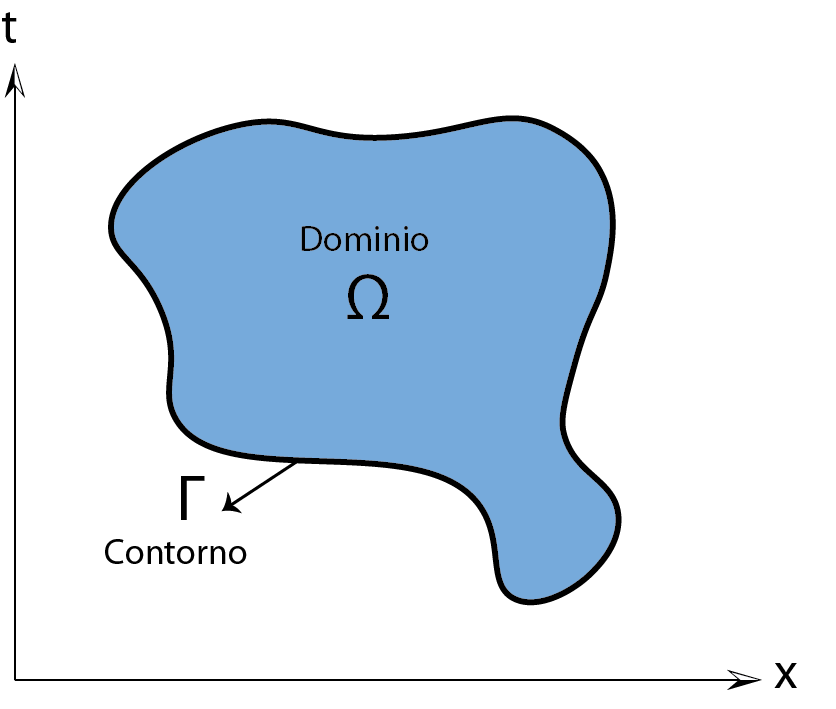
\includegraphics[width=7cm]{Imagenes/Dominio_Real.png}
        \caption{}
        \label{fig:fig32a}
\end{subfigure}
\hfill
\begin{subfigure}[b]{.45\textwidth}
        \centering
        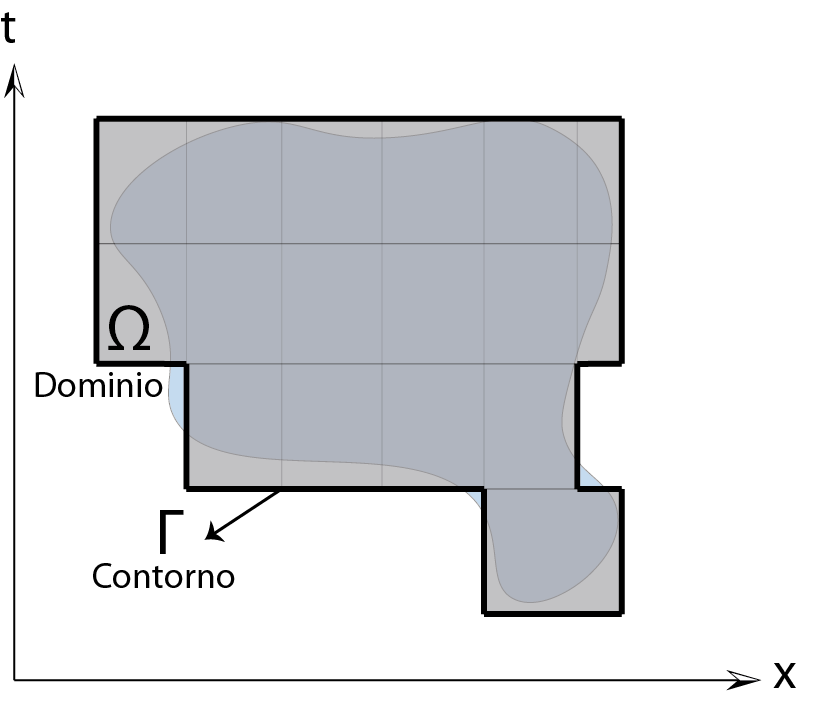
\includegraphics[width=7cm]{Imagenes/Dominio_FEM.png}
        \caption{}
        \label{fig:fig32b}
\end{subfigure}
\captionsetup{format=plain}
\caption[Dominio y contorno del modelo numérico]{Dominio y contorno del modelo numérico. (\subref{fig:fig32a}) Dominio y contorno real; (\subref{fig:fig32b}) Dominio y contorno discretizado.} 
%\vspace*{1cm}
\label{fig:fig32}
\end{figure}
%////////////////////////////////////////////////////////////////////////////////////////

Después de la integración, la \textbf{Ecuación} \textbf{\ref{eq:equ343}} queda reducida a esta ecuación diferencial ordinaria:

%----------------------------------------------------------------------------------------
% ECUACIÓN 3.44
\begin{ceqn} %\label{eq:equ344}
\begin{gather}\label{eq:equ344}
\mathbf{M}\ddot{\overline{\Phi}} + \mathbf{C}\dot{\overline{\Phi}} + \mathbf{P}(\overline{\Phi}) = 0
\end{gather}   
\end{ceqn}
%----------------------------------------------------------------------------------------

donde ($\mathbf{M}$), ($\mathbf{C}$) y ($\mathbf{P}$) son matrices o vectores cuya dimensión corresponde a la dimensión conjunto total de variables numéricas ($\overline{\Phi}_k$). Por lo general, los parámetros ($\overline{\Phi}$) representan los valores de ($\Phi^h$) en puntos llamados nodos y las funciones de forma, que generalmente son polinomios, describen la interpolación dentro de cada elemento finito, que divide el dominio ($\Omega$).\bigskip

A continuación, se discretizará en el espacio las ecuaciones geomecánicas y de flujo determinadas en el modelo matemático de la sección anterior tanto para medios porosos saturados y parcialmente saturados. En la~\MYhref[blue]{sec:sec342}{Sección 3.4.2} se hará la discretización en el tiempo del modelo geomecánico acoplado.


%........................................................................................
% TITULO DE LA SUBSECCIÓN 3.4.1.1
\subsubsection{Medio Poroso Saturado}~\hypertarget{sec:sec3411}{}
\label{sec:sec3411}

Para un medio poroso saturado con características elastoplásticas y anisotrópicas el modelo matemático es el siguiente:

%----------------------------------------------------------------------------------------
% ECUACIÓN 3.45
\begin{ceqn} 
\begin{subequations} \label{eq:equ345} 
\begin{gather}
%\begin{align}
\shortintertext{Modelo Geomecánico:} \mathbf{\nabla}(\mathbf{D}\mathbf{\nabla}\cdot\mathbf{u})-\alpha\mathbf{I}^T\mathbf{\nabla}p=\mathbf{F} \label{eq:equ345a} \\[15pt]
\shortintertext{Modelo de Flujo:} 	
\nabla^T \left[\frac{\mathbf{K}}{\mu}\nabla p\right] = \alpha\mathbf{I}^T\frac{\partial \nabla \mathbf{u}}{\partial t} +\left[\frac{\phi}{K_f}+\frac{(1-\phi)}{K_m}-\frac{\mathbf{I}\mathbf{D}\mathbf{I}^T}{(3K_{m})^{2}}\right]\frac{\partial p}{\partial t}+ q_v= 0 \label{eq:equ345b}\\[15pt]
\shortintertext{Condiciones de Contorno para presión de poros:} 	
p = \overline{p} \text{  en  } \Gamma = \Gamma_p \text{ ;  } \mathbf{n}\cdot\mathbf{w}=\mathbf{q_v} \text{  en  } \Gamma = \Gamma_w \text{ ; } \Gamma = \Gamma_p \cup \Gamma_w \label{eq:equ345c}\\[15pt]
\shortintertext{Condiciones de Contorno para desplazamiento:} 	
u = \overline{u} \text{  en  } \Gamma = \Gamma_u \text{ ;  } \mathbf{n}\cdot\mathbf{\sigma}=\mathbf{t} \text{  en  } \Gamma = \Gamma_t \text{ ; } \Gamma = \Gamma_u \cup \Gamma_t \label{eq:equ345d}
%\end{align}
\end{gather}  
\end{subequations} 
\end{ceqn}
%\bigskip
%----------------------------------------------------------------------------------------

%////////////////////////////////////////////////////////////////////////////////////////
% Figura 3.3

\begin{figure}[!ht]
\centering
\begin{subfigure}[b]{.45\textwidth}
        \centering
        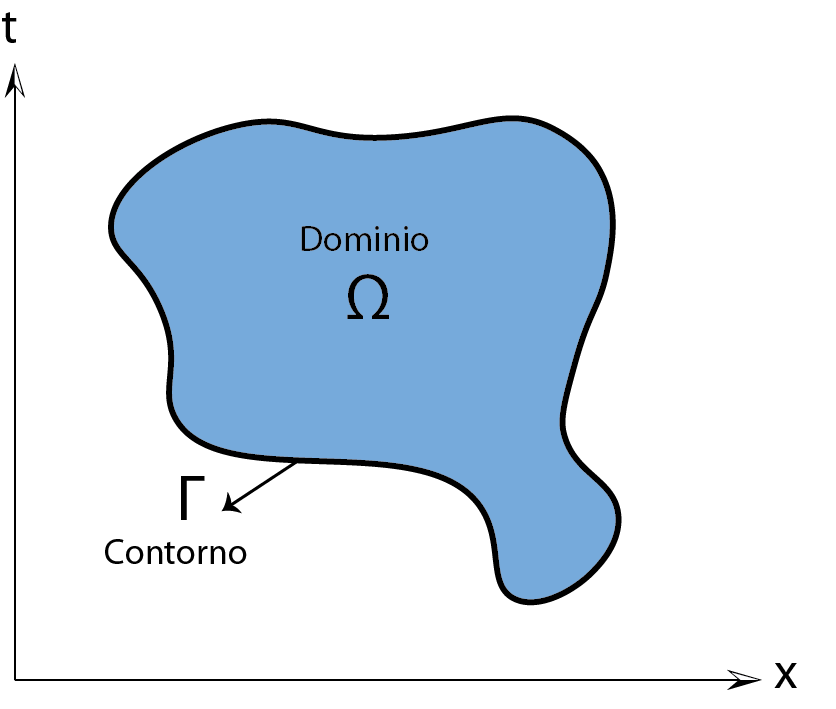
\includegraphics[width=7cm]{Imagenes/Dominio_Real.png}
        \caption{}
        \label{fig:fig33a}
\end{subfigure}
\hfill
\begin{subfigure}[b]{.45\textwidth}
        \centering
        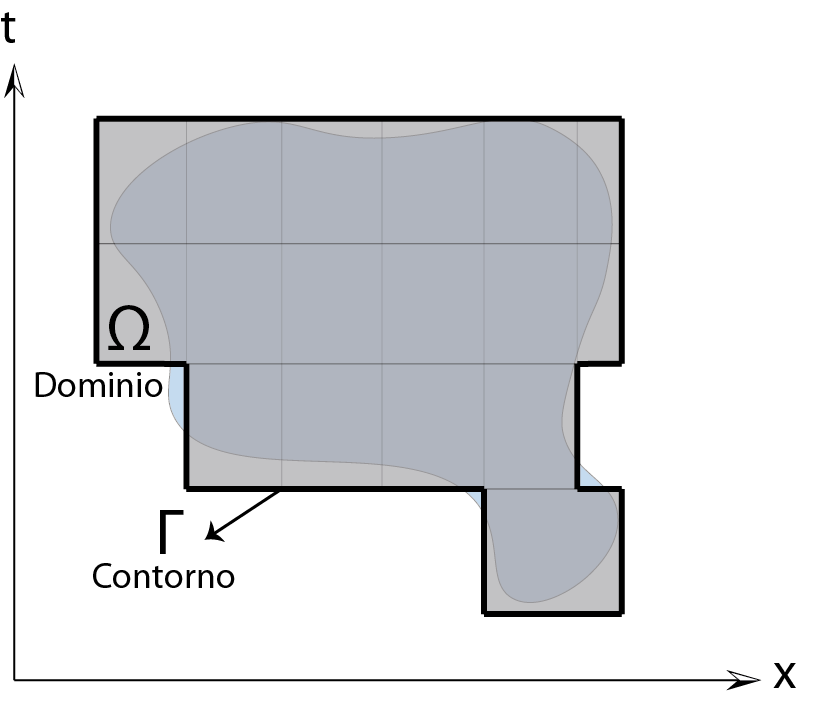
\includegraphics[width=7cm]{Imagenes/Dominio_FEM.png}
        \caption{}
        \label{fig:fig33b}
\end{subfigure}
\captionsetup{format=plain}
\caption[Dominio y contorno del modelo geomecánico acoplado]{Dominio y contorno del modelo geomecánico acoplado. (\subref{fig:fig32a}) Dominio y contorno real; (\subref{fig:fig32b}) Dominio y contorno discretizado.} 
%\vspace*{1cm}
\label{fig:fig33}
\end{figure}
%////////////////////////////////////////////////////////////////////////////////////////

Este es el modelo matemático geomecánico acoplado, que está representado por un sistema de ecuaciones diferenciales parciales donde se tienen dos incógnitas el campo de desplazamientos ($u$) y la presión de poros ($p$). Para discretizar estas ecuaciones en el dominio ($\Omega$) se asume que:

%----------------------------------------------------------------------------------------
% ECUACIÓN 3.46
\begin{ceqn} 
\begin{subequations} \label{eq:equ346} 
\begin{gather}
\mathbf{u} \cong \mathbf{u^h} = \displaystyle\sum_{k=1}^{n} N_{k}^{u} \overline{u}_k = \mathbf{N_u}\mathbf{\overline{u}}  \label{eq:equ346a}\\[12pt]
\mathbf{p} \cong \mathbf{p^h} = \displaystyle\sum_{k=1}^{n} N_{k}^{p} \overline{p}_k = \mathbf{N_p}\mathbf{\overline{p}}  \label{eq:equ346b}
\end{gather}  
\end{subequations} 
\end{ceqn}
%----------------------------------------------------------------------------------------
\\
\textbf{A. Modelo Geomecánico en Medio Poroso Saturado}
\\
Reemplazando las \textbf{Ecuaciones} \textbf{\ref{eq:equ345a}} y \textbf{\ref{eq:equ346}} en la \textbf{\ref{eq:equ343}} se obtiene:

%----------------------------------------------------------------------------------------
% ECUACIÓN 3.47
\begin{ceqn} %\label{eq:equ347}
\begin{gather}\label{eq:equ347}
\int\limits_\Omega \mathbf{N_{u}^T}\left(\mathbf{\nabla^T}(\mathbf{D}\mathbf{\nabla}\cdot[\mathbf{N_u}\mathbf{\overline{u}}])-\alpha\mathbf{I}^T\mathbf{\nabla}[\mathbf{N_p}\mathbf{\overline{p}}]-\mathbf{F}\right)\mathbf{d\Omega} = 0
\end{gather}   
\end{ceqn}
%----------------------------------------------------------------------------------------
\\
Reordenando se obtiene:

%----------------------------------------------------------------------------------------
% ECUACIÓN 3.48
\begin{ceqn} %\label{eq:equ348}
\begin{gather}\label{eq:equ348}
\int\limits_\Omega \mathbf{N_{u}^T}\mathbf{\nabla^T}\mathbf{D}\mathbf{\nabla}\mathbf{N_u}\mathbf{\overline{u}}\mathbf{d\Omega}  - \int\limits_\Omega \mathbf{N_{u}^T}\alpha\mathbf{I}^T\mathbf{\nabla}\mathbf{N_p}\mathbf{\overline{p}}\mathbf{d\Omega} - \int\limits_\Omega \mathbf{N_{u}^T}\mathbf{F}\mathbf{d\Omega} = 0
\end{gather}   
\end{ceqn}
%----------------------------------------------------------------------------------------
\\
Integrando por partes se obtiene:

%----------------------------------------------------------------------------------------
% ECUACIÓN 3.49
\begin{ceqn} %\label{eq:equ349}
\begin{gather}\label{eq:equ349}
\left[\int\limits_\Omega \mathbf{N_{u}^T}\mathbf{\nabla^T}\mathbf{D}\mathbf{\nabla}\mathbf{N_u}\mathbf{d\Omega}\right]\mathbf{\overline{u}}  - \left[\int\limits_\Omega \mathbf{N_{u}^T}\alpha\mathbf{I}^T\mathbf{\nabla}\mathbf{N_p}\mathbf{d\Omega}\right]\mathbf{\overline{p}} - \int\limits_\Omega \mathbf{N_{u}^T}\mathbf{F}\mathbf{d\Omega} = 0
\end{gather}   
\end{ceqn}
%----------------------------------------------------------------------------------------
\\
Según Zienkiewicz et al.(2013) \cite{Zienkiewicz2013TheFundamentals}:

%----------------------------------------------------------------------------------------
% ECUACIÓN 3.50
\begin{ceqn} %\label{eq:equ350}
\begin{gather}\label{eq:equ350}
\mathbf{B} = \mathbf{\nabla N_u}
\end{gather}   
\end{ceqn}
%----------------------------------------------------------------------------------------

Por lo tanto, la \textbf{Ecuación} \textbf{\ref{eq:equ349}} se transforma en:

%----------------------------------------------------------------------------------------
% ECUACIÓN 3.51
\begin{ceqn} %\label{eq:equ351}
\begin{gather}\label{eq:equ351}
\left[\int\limits_\Omega \mathbf{B^T}\mathbf{D}\mathbf{B}\mathbf{d\Omega}\right]\mathbf{\overline{u}}  - \left[\int\limits_\Omega \mathbf{B^T}\alpha\mathbf{I}^T\mathbf{N_p}\mathbf{d\Omega}\right]\mathbf{\overline{p}} - \int\limits_\Omega \mathbf{N_{u}^T}\mathbf{F}\mathbf{d\Omega} = 0
\end{gather}   
\end{ceqn}
%----------------------------------------------------------------------------------------
\\
Es decie que el modelo numérico geomecánico para un medio saturado es:

%----------------------------------------------------------------------------------------
% ECUACIÓN 3.52
\begin{ceqn} 
\begin{subequations} \label{eq:equ352} 
\begin{gather}
\mathbf{M}\mathbf{\overline{u}} - \mathbf{C}\mathbf{\overline{p}} = \mathbf{f_u}\label{eq:equ352a}\\[12pt]
\mathbf{M} = \int\limits_\Omega \mathbf{B^T}\mathbf{D}\mathbf{B}\mathbf{d\Omega} \label{eq:equ352b}\\[12pt]
\mathbf{C} =  \int\limits_\Omega \mathbf{B^T}\alpha\mathbf{I}^T\mathbf{N_p}\mathbf{d\Omega} \label{eq:equ352c}\\[12pt]
\mathbf{f_u} = \int\limits_\Omega \mathbf{N_{u}^T}\mathbf{F}\mathbf{d\Omega} + \oint\limits_{\Gamma_{t}}  \mathbf{N_{u}^T} \overline{t} \mathbf{d\Gamma} \label{eq:equ352d}\\[12pt]
u = \overline{u} \text{  en  } \Gamma = \Gamma_u \text{ ;  } \mathbf{n}\cdot\mathbf{\sigma}=\mathbf{t} \text{  en  } \Gamma = \Gamma_t \text{ ; } \Gamma = \Gamma_u \cup \Gamma_t \label{eq:equ352e}
\end{gather}  
\end{subequations} 
\end{ceqn}
%----------------------------------------------------------------------------------------

\bigskip
\textbf{B. Modelo de Flujo en Medio Poroso Saturado}\\
Reemplazando las \textbf{Ecuaciones} \textbf{\ref{eq:equ345b}} y \textbf{\ref{eq:equ346}} en la \textbf{\ref{eq:equ343}} se obtiene:\bigskip

%----------------------------------------------------------------------------------------
% ECUACIÓN 3.53
\begin{ceqn} 
\begin{subequations} \label{eq:equ353} 
\begin{gather}
\int\limits_\Omega \mathbf{N_{p}^T}\left( \nabla^T \left[\frac{\mathbf{K}}{\mu}\nabla [\mathbf{N_p}\mathbf{\overline{p}}]\right] - \alpha\mathbf{I}^T\frac{\partial \nabla [\mathbf{N_u}\mathbf{\overline{u}}]}{\partial t} -\frac{1}{Q}\frac{\partial [\mathbf{N_p}\mathbf{\overline{p}}]}{\partial t} - q_v\right)\mathbf{d\Omega} = 0 \label{eq:equ353a} \\[12pt]
\frac{1}{Q}=\frac{\phi}{K_f}+\frac{(1-\phi)}{K_m}-\frac{\mathbf{I}\mathbf{D}\mathbf{I}^T}{(3K_{m})^{2}} \label{eq:equ353b}
\end{gather}  
\end{subequations} 
\end{ceqn}
%----------------------------------------------------------------------------------------
\\
Reordenando se obtiene:

%----------------------------------------------------------------------------------------
% ECUACIÓN 3.54
\begin{ceqn} 
\begin{gather}\label{eq:equ354} 
\int\limits_\Omega \nabla^T\mathbf{N_{p}^T} \frac{\mathbf{K}}{\mu}\nabla \mathbf{N_p}\mathbf{\overline{p}} \mathbf{d\Omega} - \int\limits_\Omega \mathbf{N_{p}^T}\alpha\mathbf{I}^T\nabla\mathbf{N_u}\frac{\partial \mathbf{\overline{u}}}{\partial t} \mathbf{d\Omega}  -\int\limits_\Omega \mathbf{N_{p}^T}\frac{1}{Q}\mathbf{N_p}\frac{\partial \mathbf{\overline{p}}}{\partial t} 
- \int\limits_\Omega \mathbf{N_{p}^T} q_v \mathbf{d\Omega} = 0
\end{gather}  
\end{ceqn}
%----------------------------------------------------------------------------------------
\\
Integrando por partes resulta:

%----------------------------------------------------------------------------------------
% ECUACIÓN 3.55
\begin{ceqn} 
\begin{gather}\label{eq:equ355} 
\left[\int\limits_\Omega \nabla^T\mathbf{N_{p}^T} \frac{\mathbf{K}}{\mu}\nabla \mathbf{N_p} \mathbf{d\Omega}\right]\mathbf{\overline{p}} - \left[\int\limits_\Omega \mathbf{N_{p}^T}\alpha\mathbf{I}^T\nabla\mathbf{N_u} \mathbf{d\Omega}\right]\frac{\partial \mathbf{\overline{u}}}{\partial t}  -\left[\int\limits_\Omega \mathbf{N_{p}^T}\frac{1}{Q}\mathbf{N_p}\right]\frac{\partial \mathbf{\overline{p}}}{\partial t}
- \int\limits_\Omega \mathbf{N_{p}^T} q_v \mathbf{d\Omega} = 0
\end{gather}  
\end{ceqn}
%--------------------------------------------------------------------------------------
\\
Por lo tanto, el modelo de flujo para un medio saturado es:

%--------------------------------------------------------------------------------------
% ECUACIÓN 3.56
\begin{ceqn} 
\begin{subequations} \label{eq:equ356} 
\begin{gather}
\mathbf{H}\mathbf{\overline{p}} + \mathbf{C^T}\frac{\partial \mathbf{\overline{u}}}{\partial t} +\mathbf{S}\frac{\partial \mathbf{\overline{p}}}{\partial t} = \mathbf{f_p}\label{eq:equ356a}\\[12pt]
\mathbf{H} = \int\limits_\Omega \mathbf{B^T}\frac{\mathbf{K}}{\mu}\mathbf{B}\mathbf{d\Omega} \label{eq:equ356b}\\[12pt]
\mathbf{C^T} =  \int\limits_\Omega \mathbf{N_p^T}\alpha\mathbf{I}^T\mathbf{B}\mathbf{d\Omega} \label{eq:equ356c}\\[12pt]
\mathbf{S} =  \int\limits_\Omega \mathbf{N_p^T}\frac{1}{Q}\mathbf{N_p}\mathbf{d\Omega} \label{eq:equ356d}\\[12pt]
\mathbf{f_p} = \int\limits_\Omega \mathbf{N_{p}^T}\mathbf{q_v}\mathbf{d\Omega} + \oint\limits_{\Gamma_{w}}  \mathbf{N_{p}^T} \overline{w} \mathbf{d\Gamma} \label{eq:equ356e}\\[12pt]
p = \overline{p} \text{  en  } \Gamma = \Gamma_p \text{ ;  } \mathbf{n}\cdot\mathbf{w}=\mathbf{q_v} \text{  en  } \Gamma = \Gamma_w \text{ ; } \Gamma = \Gamma_p \cup \Gamma_w \label{eq:equ356f}
\end{gather}  
\end{subequations} 
\end{ceqn}
%--------------------------------------------------------------------------------------

\textbf{C. Modelo Totalmente Acoplado en Medio Poroso Saturado}\\
La discretización en elementos finitos del modelo geomecánico totalmente acoplado para un medio poroso saturado, que se expuso en la \textbf{Ecuación} \textbf{\ref{eq:equ345}} se puede expresar de la siguiente manera:\bigskip

%--------------------------------------------------------------------------------------
% ECUACIÓN 3.57
\begin{ceqn} %\label{eq:equ357}
\begin{subequations}\label{eq:equ357}
\begin{gather}
\begin{bmatrix}
       \mathbf{M}  & \mathbf{-C}   \\[0.3em]
       0		   & \mathbf{H}       		
\end{bmatrix}
\begin{Bmatrix}
       \mathbf{\overline{u}}    \\[0.3em]
       \mathbf{\overline{p}}      		
\end{Bmatrix}
+
\begin{bmatrix}
       0             & 0           \\[0.3em]
       \mathbf{C}^T  & \mathbf{S}       		
\end{bmatrix}
\begin{Bmatrix}
       \mathbf{\dot{\overline{u}}}    \\[0.3em]
       \mathbf{\dot{\overline{p}}}      		
\end{Bmatrix}
= 
\begin{Bmatrix}
       \mathbf{f_u}    \\[0.3em]
       \mathbf{f_p}      		
\end{Bmatrix} \label{eq:equ357a}\\[12pt]
u = \overline{u} \text{  en  } \Gamma = \Gamma_u \text{ ;  } \mathbf{n}\cdot\mathbf{\sigma}=\mathbf{t} \text{  en  } \Gamma = \Gamma_t \text{ ; } \Gamma = \Gamma_u \cup \Gamma_t \label{eq:equ357b}\\[12pt]
p = \overline{p} \text{  en  } \Gamma = \Gamma_p \text{ ;  } \mathbf{n}\cdot\mathbf{w}=\mathbf{q_v} \text{  en  } \Gamma = \Gamma_w \text{ ; } \Gamma = \Gamma_p \cup \Gamma_w \label{eq:equ357c}
\end{gather}
\end{subequations}
\end{ceqn}
%--------------------------------------------------------------------------------------

donde ($\mathbf{M}$) es la matriz de rigidez elástica, ($\mathbf{C}$) es la matriz de acoplamiento, ($\mathbf{H}$) es la matriz de rigidez de flujo, ($\mathbf{S}$) es la matriz de capacidad de flujo, $[\mathbf{\overline{u}}, \mathbf{\overline{p}} ]^T$ es el vector de incógnitas (i.e. desplazamientos y presiones de poros),  $[\mathbf{\dot{\overline{u}}},\mathbf{\dot{\overline{p}}} ]^T$ es el vector de las derivadas en el tiempo (i.e. $\partial \mathbf{\overline{u}}/\partial t$, $\partial \mathbf{\overline{p}}/\partial t$), $[\mathbf{f_u}, \mathbf{f_p} ]^T$ es el vector de cargas nodales y fuentes de flujo.\bigskip


%........................................................................................
% TITULO DE LA SUBSECCIÓN 3.4.1.2
\subsubsection{Medio Poroso Parcialmente Saturado}~\hypertarget{sec:sec3412}{}
\label{sec:sec3412}

Para un medio poroso parcialmente saturado con características elastoplásticas y anisotrópicas el modelo matemático es el siguiente:

%----------------------------------------------------------------------------------------
% ECUACIÓN 3.58
\begin{ceqn} 
\begin{subequations} \label{eq:equ358} 
\begin{gather}
%\begin{align}
\shortintertext{Modelo geomecánico:} \mathbf{\nabla^T}(\mathbf{D}\mathbf{\nabla}\cdot\mathbf{u})-\alpha\mathbf{I}^TS''_w\mathbf{\nabla}p_w -\alpha\mathbf{I}^TS''_n\mathbf{\nabla}p_n=\mathbf{F} \label{eq:equ358a} \\[10pt]
S''_w = S_w + P_c\frac{\partial S_w}{\partial P_c}  \label{eq:equ358b} \\[10pt]
S''_n = S_n - P_c\frac{\partial S_n}{\partial P_c}  \label{eq:equ358c} \\[8pt]
P_c = \mathnormal{f}(S_w) = p_n - p_w  \label{eq:equ358d} \\[8pt]
\shortintertext{Modelo de flujo para el fluido mojado:} 	
\begin{multlined}
\nabla^T \left[\frac{k k_{rw}}{\mu_{w}}\nabla p_w\right] = \left[S_w \frac{\alpha - \phi}{K_m}S''_w + \phi\frac{S_w}{K_w} - \phi\frac{\partial S_w}{\partial P_c}\right]\frac{\partial p_w}{\partial t} \\[10pt]
+ \left[S_w \frac{\alpha - \phi}{K_m}S''_n + \phi\frac{\partial S_w}{\partial P_c}\right]\frac{\partial p_n}{\partial t} +\alpha S_w\mathbf{I}^T\frac{\partial \nabla \mathbf{u}}{\partial t} + q_w\end{multlined} \label{eq:equ358e}\\[10pt]
S''_w = S_w + P_c\frac{\partial S_w}{\partial P_c}  \label{eq:equ358f}\\[8pt]
S''_n = S_n - P_c\frac{\partial S_w}{\partial P_c}  \label{eq:equ358g}\\[8pt]
\shortintertext{Modelo de flujo para el fluido no-mojado:} 	
\begin{multlined}
\nabla^T \left[\frac{k k_{rw}}{\mu_{w}}\nabla p_w\right] = \left[S_w \frac{\alpha - \phi}{K_m}S''_w + \phi\frac{S_w}{K_w} - \phi\frac{\partial S_w}{\partial P_c}\right]\frac{\partial p_w}{\partial t} \\[10pt]
+ \left[S_w \frac{\alpha - \phi}{K_m}S''_n + \phi\frac{\partial S_w}{\partial P_c}\right]\frac{\partial p_n}{\partial t} +\alpha S_w\mathbf{I}^T\frac{\partial \nabla \mathbf{u}}{\partial t} + q_w\end{multlined} \label{eq:equ358h}\\[10pt]
S''_w = S_w + P_c\frac{\partial S_w}{\partial P_c}  \label{eq:equ358i}\\[8pt]
S''_n = S_n - P_c\frac{\partial S_w}{\partial P_c}  \label{eq:equ358j}\\[8pt]
\shortintertext{Condiciones de contorno para presión de poros:} 	
p = \overline{p} \text{  en  } \Gamma = \Gamma_p \text{ ;  } \mathbf{n}\cdot\mathbf{w}=\mathbf{q_v} \text{  en  } \Gamma = \Gamma_w \text{ ; } \Gamma = \Gamma_p \cup \Gamma_w \label{eq:equ358k}\\[8pt]
\shortintertext{Condiciones de contorno para desplazamiento:} 	
u = \overline{u} \text{  en  } \Gamma = \Gamma_u \text{ ;  } \mathbf{n}\cdot\mathbf{\sigma}=\mathbf{t} \text{  en  } \Gamma = \Gamma_t \text{ ; } \Gamma = \Gamma_u \cup \Gamma_t \label{eq:equ358l}
%\end{align}
\end{gather}  
\end{subequations} 
\end{ceqn}
%\bigskip
%----------------------------------------------------------------------------------------

Este es el modelo matemático geomecánico acoplado, representado por un sistema de ecuaciones diferenciales parciales donde se tienen tres incógnitas el campo de desplazamientos ($u$), la presión de poros del fluido mojado($p_w$) y la presión de poros del fluido no-mojado($p_n$). Para discretizar estas ecuaciones en el dominio ($\Omega$) se asume que:

%----------------------------------------------------------------------------------------
% ECUACIÓN 3.59
\begin{ceqn} 
\begin{subequations} \label{eq:equ359} 
\begin{gather}
\mathbf{u} \cong \mathbf{u^h} = \displaystyle\sum_{k=1}^{n} N_{k}^{u} \overline{u}_k = \mathbf{N_u}\mathbf{\overline{u}}  \label{eq:equ359a}\\[12pt]
\mathbf{p_w} \cong \mathbf{p_{w}^h} = \displaystyle\sum_{k=1}^{n} N_{k}^{p} \overline{p^w}_k = \mathbf{N_p}\mathbf{\overline{p_w}}  \label{eq:equ359b}\\[12pt]
\mathbf{p_n} \cong \mathbf{p_{n}^h} = \displaystyle\sum_{k=1}^{n} N_{k}^{p} \overline{p^n}_k = \mathbf{N_p}\mathbf{\overline{p_n}}  \label{eq:equ359c}
\end{gather}  
\end{subequations} 
\end{ceqn}
%----------------------------------------------------------------------------------------

\bigskip
\textbf{A. Modelo Geomecánico en Medio Poroso Parcialmente Saturado}\\
Reemplazando las \textbf{Ecuaciones} \textbf{\ref{eq:equ358a}} y \textbf{\ref{eq:equ359}} en la \textbf{\ref{eq:equ343}} se obtiene:\bigskip

%----------------------------------------------------------------------------------------
% ECUACIÓN 3.60
\begin{ceqn} %\label{eq:equ360}
\begin{gather}\label{eq:equ360}
\int\limits_\Omega \mathbf{N_{u}^T}\left(\mathbf{\nabla^T}(\mathbf{D}\mathbf{\nabla}\cdot[\mathbf{N_u}\mathbf{\overline{u}}])-\alpha\mathbf{I}^TS''_w\mathbf{\nabla}[\mathbf{N_p}\mathbf{\overline{p_w}}] -\alpha\mathbf{I}^TS''_n\mathbf{\nabla}[\mathbf{N_p}\mathbf{\overline{p_n}}] - \mathbf{F}\right)\mathbf{d\Omega} = 0
\end{gather}   
\end{ceqn}
%----------------------------------------------------------------------------------------
\bigskip
Reordenando se obtiene:

%----------------------------------------------------------------------------------------
% ECUACIÓN 3.61
\begin{ceqn} %\label{eq:equ361}
\begin{gather}\label{eq:equ361}
\begin{multlined}
\int\limits_\Omega \mathbf{N_{u}^T}\mathbf{\nabla^T}\mathbf{D}\mathbf{\nabla}\mathbf{N_u}\mathbf{\overline{u}}\mathbf{d\Omega} - \int\limits_\Omega \mathbf{N_{u}^T} \alpha\mathbf{I}^TS''_w\mathbf{\nabla}\mathbf{N_p}\mathbf{\overline{p_w}}\mathbf{d\Omega}\\[12pt] -\int\limits_\Omega \mathbf{N_{u}^T} \alpha\mathbf{I}^TS''_n\mathbf{\nabla}\mathbf{N_p}\mathbf{\overline{p_n}}\mathbf{d\Omega} - \int\limits_\Omega \mathbf{N_{u}^T} \mathbf{F}\mathbf{d\Omega} = 0
\end{multlined}
\end{gather}   
\end{ceqn}
%----------------------------------------------------------------------------------------

\bigskip
Integrando por partes la \textbf{\ref{eq:equ361}} se obtiene:\bigskip

%----------------------------------------------------------------------------------------
% ECUACIÓN 3.62
\begin{ceqn} %\label{eq:equ362}
\begin{gather}\label{eq:equ362}
\begin{multlined}
\left[\int\limits_\Omega \mathbf{N_{u}^T}\mathbf{\nabla^T}\mathbf{D}\mathbf{\nabla}\mathbf{N_u}\mathbf{d\Omega}\right]\mathbf{\overline{u}} - \left[\int\limits_\Omega \mathbf{N_{u}^T} \alpha\mathbf{I}^TS''_w\mathbf{\nabla}\mathbf{N_p}\mathbf{d\Omega}\right]\mathbf{\overline{p_w}}\\[12pt] 
- \left[\int\limits_\Omega \mathbf{N_{u}^T}\alpha\mathbf{I}^TS''_n\mathbf{\nabla}\mathbf{N_p}\mathbf{d\Omega}\right]\mathbf{\overline{p_n}} - \int\limits_\Omega \mathbf{N_{u}^T} \mathbf{F}\mathbf{d\Omega} = 0
\end{multlined}
\end{gather}   
\end{ceqn}
%----------------------------------------------------------------------------------------
\\
Según Zienkiewicz et al.(2013) \cite{Zienkiewicz2013TheFundamentals}:

%----------------------------------------------------------------------------------------
% ECUACIÓN 3.63
\begin{ceqn} %\label{eq:equ363}
\begin{gather}\label{eq:equ63}
\mathbf{B} = \mathbf{\nabla N_u}
\end{gather}   
\end{ceqn}
%----------------------------------------------------------------------------------------
\\
Por tanto, la \textbf{Ecuación} \textbf{\ref{eq:equ362}} se transforma en:

%----------------------------------------------------------------------------------------
% ECUACIÓN 3.64
\begin{ceqn} %\label{eq:equ364}
\begin{gather}\label{eq:equ364}
\begin{multlined}
\left[\int\limits_\Omega \mathbf{B^T}\mathbf{D}\mathbf{B}\mathbf{d\Omega}\right]\mathbf{\overline{u}} - \left[\int\limits_\Omega \mathbf{B^T} \alpha\mathbf{I}^TS''_w\mathbf{\nabla}\mathbf{N_p}\mathbf{d\Omega}\right]\mathbf{\overline{p_w}}\\[12pt] 
- \left[\int\limits_\Omega \mathbf{B^T}\alpha\mathbf{I}^TS''_n\mathbf{\nabla}\mathbf{N_p}\mathbf{d\Omega}\right]\mathbf{\overline{p_n}} - \int\limits_\Omega \mathbf{N_{u}^T} \mathbf{F}\mathbf{d\Omega} = 0
\end{multlined}
\end{gather}   
\end{ceqn}
%----------------------------------------------------------------------------------------
\bigskip
Es decir que  el modelo numérico geomecánico para un medio parcialmente saturado es:

%----------------------------------------------------------------------------------------
% ECUACIÓN 3.65
\begin{ceqn} 
\begin{subequations} \label{eq:equ365} 
\begin{gather}
\mathbf{M}\mathbf{\overline{u}} - \mathbf{C_{sw}}\mathbf{\overline{p_w}} - \mathbf{C_{sn}}\mathbf{\overline{p_n}} = \mathbf{f_u}\label{eq:equ365a}\\[12pt]
\mathbf{M} = \int\limits_\Omega \mathbf{B^T}\mathbf{D}\mathbf{B}\mathbf{d\Omega} \label{eq:equ365b}\\[12pt]
\mathbf{C_{sw}} =  \int\limits_\Omega \mathbf{B^T} \alpha\mathbf{I}^TS''_w\mathbf{\nabla}\mathbf{N_p}\mathbf{d\Omega} \label{eq:equ365c}\\[12pt]
\mathbf{C_{sn}} =  \int\limits_\Omega \mathbf{B^T} \alpha\mathbf{I}^TS''_n\mathbf{\nabla}\mathbf{N_p}\mathbf{d\Omega} \label{eq:equ365d}\\[12pt]
\mathbf{f_u} = \int\limits_\Omega \mathbf{N_{u}^T}\mathbf{F}\mathbf{d\Omega} + \oint\limits_{\Gamma_{t}}  \mathbf{N_{u}^T} \overline{t} \mathbf{d\Gamma} \label{eq:equ365e}\\[12pt]
u = \overline{u} \text{  en  } \Gamma = \Gamma_u \text{ ;  } \mathbf{n}\cdot\mathbf{\sigma}=\mathbf{t} \text{  en  } \Gamma = \Gamma_t \text{ ; } \Gamma = \Gamma_u \cup \Gamma_t \label{eq:equ365f}
\end{gather}  
\end{subequations} 
\end{ceqn}
%----------------------------------------------------------------------------------------

\bigskip
\textbf{B. Modelo de Flujo para fluido mojado}\\
Reemplazando las \textbf{Ecuaciones} \textbf{\ref{eq:equ358e}} y \textbf{\ref{eq:equ359}} en la \textbf{\ref{eq:equ343}} se obtiene:\bigskip

%----------------------------------------------------------------------------------------
% ECUACIÓN 3.66
\begin{ceqn} 
\begin{subequations} \label{eq:equ366} 
\begin{gather}
\begin{multlined}
\int\limits_\Omega \mathbf{N_{p}^T}\left( \nabla^T \left[\frac{k k_{rw}}{\mu_{w}}\nabla [\mathbf{N_p}\mathbf{\overline{p_w}}] \right] + \frac{1}{Q_{ww}}\frac{\partial [\mathbf{N_p}\mathbf{\overline{p_w}}]}{\partial t} \right. \\[12pt]
\left. {} + \frac{1}{Q_{wn}}\frac{\partial [\mathbf{N_p}\mathbf{\overline{p_n}}]}{\partial t} +\alpha S_w\mathbf{I}^T\frac{\partial \nabla [\mathbf{N_u}\mathbf{\overline{u}}]}{\partial t} + q_w\right) \mathbf{d\Omega} = 0 \end{multlined}\label{eq:equ366a}\\[12pt]
\frac{1}{Q_{ww}} = S_w \frac{\alpha - \phi}{K_m}S''_w + \phi\frac{S_w}{K_w} - \phi\frac{\partial S_w}{\partial P_c} \label{eq:equ66b}\\[12pt]
\frac{1}{Q_{wn}} = S_w \frac{\alpha - \phi}{K_m}S''_n + \phi\frac{\partial S_w}{\partial P_c} \label{eq:equ66c}
\end{gather}  
\end{subequations} 
\end{ceqn}
%----------------------------------------------------------------------------------------

\bigskip
Reordenando se obtiene:

%----------------------------------------------------------------------------------------
% ECUACIÓN 3.67
\begin{ceqn} 
\begin{gather} \label{eq:equ367} 
\begin{multlined}
\int\limits_\Omega \nabla^T\mathbf{N_{p}^T} \frac{k k_{rw}}{\mu_{w}}\nabla \mathbf{N_p}\mathbf{\overline{p_w}} \mathbf{d\Omega}  + \int\limits_\Omega \mathbf{N_{p}^T}\frac{1}{Q_{ww}}\mathbf{N_p}\frac{\partial \mathbf{\overline{p_w}}}{\partial t}\mathbf{d\Omega}\\[12pt] 
+ \int\limits_\Omega \mathbf{N_{p}^T}\frac{1}{Q_{wn}}\mathbf{N_p}\frac{\partial \mathbf{\overline{p_n}}}{\partial t}\mathbf{d\Omega} + \int\limits_\Omega \mathbf{N_{p}^T}\alpha S_w\mathbf{I}^T\mathbf{N_u}\frac{\partial \nabla \mathbf{\overline{u}}}{\partial t}\mathbf{d\Omega} + \int\limits_\Omega \mathbf{N_{p}^T}q_w \mathbf{d\Omega} = 0
\end{multlined}
\end{gather} 
\end{ceqn}
%----------------------------------------------------------------------------------------

\bigskip
Integrando por partes la \textbf{\ref{eq:equ367}} se obtiene:\bigskip

%----------------------------------------------------------------------------------------
% ECUACIÓN 3.68
\begin{ceqn} 
\begin{gather} \label{eq:equ368} 
\begin{multlined}
\left[\int\limits_\Omega \nabla^T\mathbf{N_{p}^T} \frac{k k_{rw}}{\mu_{w}}\nabla \mathbf{N_p} \mathbf{d\Omega}\right]\mathbf{\overline{p_w}}  + \left[\int\limits_\Omega \mathbf{N_{p}^T}\frac{1}{Q_{ww}}\mathbf{N_p}\mathbf{d\Omega}\right]\frac{\partial \mathbf{\overline{p_w}}}{\partial t}\\[12pt] 
+ \left[\int\limits_\Omega \mathbf{N_{p}^T}\frac{1}{Q_{wn}}\mathbf{N_p}\mathbf{d\Omega}\right]\frac{\partial \mathbf{\overline{p_n}}}{\partial t} + \left[\int\limits_\Omega \mathbf{N_{p}^T}\alpha S_w\mathbf{I}^T\nabla\mathbf{N_u}\mathbf{d\Omega}\right]\frac{\partial  \mathbf{\overline{u}}}{\partial t} + \int\limits_\Omega \mathbf{N_{p}^T}q_w \mathbf{d\Omega} = 0
\end{multlined}
\end{gather} 
\end{ceqn}
%----------------------------------------------------------------------------------------

\bigskip
Por lo tanto, el modelo de flujo para el fluido mojado:

%--------------------------------------------------------------------------------------
% ECUACIÓN 3.69
\begin{ceqn} 
\begin{subequations} \label{eq:equ369} 
\begin{gather}
\mathbf{H_{ww}}\mathbf{\overline{p_w}} + \mathbf{C_{ws}}\frac{\partial \mathbf{\overline{u}}}{\partial t} + \mathbf{S_{ww}}\frac{\partial \mathbf{\overline{p_w}}}{\partial t} + \mathbf{C_{wn}}\frac{\partial \mathbf{\overline{p_n}}}{\partial t} = \mathbf{f_w}\label{eq:equ369a}\\[12pt]
\mathbf{H_{ww}} = \int\limits_\Omega \mathbf{B^T} \frac{k k_{rw}}{\mu_{w}}\mathbf{B}\mathbf{d\Omega} \label{eq:equ369b}\\[12pt]
\mathbf{C_{ws}} =  \int\limits_\Omega \mathbf{N_{p}^T}\alpha S_w\mathbf{I}^T\mathbf{B}\mathbf{d\Omega} \label{eq:equ369c}\\[12pt]
\mathbf{S_{ww}} =  \int\limits_\Omega \mathbf{N_p^T}\frac{1}{Q_{ww}}\mathbf{N_p}\mathbf{d\Omega} \label{eq:equ369d}\\[12pt]
\mathbf{C_{wn}} =  \int\limits_\Omega \mathbf{N_p^T}\frac{1}{Q_{wn}}\mathbf{N_p}\mathbf{d\Omega} \label{eq:equ369e}\\[12pt]
\mathbf{f_w} = \int\limits_\Omega \mathbf{N_{p}^T}q_w\mathbf{d\Omega} + \oint\limits_{\Gamma_{w}}  \mathbf{N_{p}^T} \overline{w} \mathbf{d\Gamma} \label{eq:equ369f}\\[12pt]
p = \overline{p} \text{  en  } \Gamma = \Gamma_p \text{ ;  } \mathbf{n}\cdot\mathbf{w}=\mathbf{q_v} \text{  en  } \Gamma = \Gamma_w \text{ ; } \Gamma = \Gamma_p \cup \Gamma_w \label{eq:equ369g}
\end{gather}  
\end{subequations} 
\end{ceqn}
%--------------------------------------------------------------------------------------

\bigskip
\textbf{C. Modelo de Flujo para fluido no-mojado}\\
Reemplazando las \textbf{Ecuaciones} \textbf{\ref{eq:equ358h}} y \textbf{\ref{eq:equ359}} en la \textbf{\ref{eq:equ343}} se obtiene:\bigskip

%----------------------------------------------------------------------------------------
% ECUACIÓN 3.70
\begin{ceqn} 
\begin{subequations} \label{eq:equ370} 
\begin{gather}
\begin{multlined}
\int\limits_\Omega \mathbf{N_{p}^T}\left( \nabla^T \left[\frac{k k_{rn}}{\mu_{n}}\nabla [\mathbf{N_p}\mathbf{\overline{p_n}}] \right] + \frac{1}{Q_{nn}}\frac{\partial [\mathbf{N_p}\mathbf{\overline{p_n}}]}{\partial t} \right. \\[12pt]
\left. {} + \frac{1}{Q_{nw}}\frac{\partial [\mathbf{N_p}\mathbf{\overline{p_w}}]}{\partial t} +\alpha S_n\mathbf{I}^T\frac{\partial \nabla [\mathbf{N_u}\mathbf{\overline{u}}]}{\partial t} + q_w\right) \mathbf{d\Omega} = 0 \end{multlined}\label{eq:equ370a}\\[12pt]
\frac{1}{Q_{nn}} = S_n \frac{\alpha - \phi}{K_m}S''_n + \phi\frac{S_n}{K_n} - \phi\frac{\partial S_w}{\partial P_c} \label{eq:equ70b}\\[12pt]
\frac{1}{Q_{nw}} = S_n \frac{\alpha - \phi}{K_m}S''_w + \phi\frac{\partial S_w}{\partial P_c} \label{eq:equ70c}
\end{gather}  
\end{subequations} 
\end{ceqn}
%----------------------------------------------------------------------------------------

\bigskip
Reordenando se obtiene:

%----------------------------------------------------------------------------------------
% ECUACIÓN 3.71
\begin{ceqn} 
\begin{gather} \label{eq:equ371} 
\begin{multlined}
\int\limits_\Omega \nabla^T\mathbf{N_{p}^T} \frac{k k_{rn}}{\mu_{n}}\nabla \mathbf{N_p}\mathbf{\overline{p_n}} \mathbf{d\Omega}  + \int\limits_\Omega \mathbf{N_{p}^T}\frac{1}{Q_{nn}}\mathbf{N_p}\frac{\partial \mathbf{\overline{p_n}}}{\partial t}\mathbf{d\Omega}\\[12pt] 
+ \int\limits_\Omega \mathbf{N_{p}^T}\frac{1}{Q_{nw}}\mathbf{N_p}\frac{\partial \mathbf{\overline{p_w}}}{\partial t}\mathbf{d\Omega} + \int\limits_\Omega \mathbf{N_{p}^T}\alpha S_n\mathbf{I}^T\mathbf{N_u}\frac{\partial \nabla \mathbf{\overline{u}}}{\partial t}\mathbf{d\Omega} + \int\limits_\Omega \mathbf{N_{p}^T}q_w \mathbf{d\Omega} = 0
\end{multlined}
\end{gather} 
\end{ceqn}
%----------------------------------------------------------------------------------------

\bigskip
Integrando por partes la \textbf{\ref{eq:equ371}} se obtiene:\bigskip

%----------------------------------------------------------------------------------------
% ECUACIÓN 3.72
\begin{ceqn} 
\begin{gather} \label{eq:equ372} 
\begin{multlined}
\left[\int\limits_\Omega \nabla^T\mathbf{N_{p}^T} \frac{k k_{rn}}{\mu_{n}}\nabla \mathbf{N_p} \mathbf{d\Omega}\right]\mathbf{\overline{p_n}}  + \left[\int\limits_\Omega \mathbf{N_{p}^T}\frac{1}{Q_{nn}}\mathbf{N_p}\mathbf{d\Omega}\right]\frac{\partial \mathbf{\overline{p_n}}}{\partial t}\\[12pt] 
+ \left[\int\limits_\Omega \mathbf{N_{p}^T}\frac{1}{Q_{nw}}\mathbf{N_p}\mathbf{d\Omega}\right]\frac{\partial \mathbf{\overline{p_w}}}{\partial t} + \left[\int\limits_\Omega \mathbf{N_{p}^T}\alpha S_n\mathbf{I}^T\nabla\mathbf{N_u}\mathbf{d\Omega}\right]\frac{\partial  \mathbf{\overline{u}}}{\partial t} + \int\limits_\Omega \mathbf{N_{p}^T}q_n \mathbf{d\Omega} = 0
\end{multlined}
\end{gather} 
\end{ceqn}
%----------------------------------------------------------------------------------------

\bigskip
Por lo tanto, el modelo de flujo para el fluido mojado:

%--------------------------------------------------------------------------------------
% ECUACIÓN 3.73
\begin{ceqn} 
\begin{subequations} \label{eq:equ373} 
\begin{gather}
\mathbf{H_{nn}}\mathbf{\overline{p_w}} + \mathbf{C_{ns}}\frac{\partial \mathbf{\overline{u}}}{\partial t} + \mathbf{S_{nn}}\frac{\partial \mathbf{\overline{p_w}}}{\partial t} + \mathbf{C_{nw}}\frac{\partial \mathbf{\overline{p_n}}}{\partial t} = \mathbf{f_n}\label{eq:equ373a}\\[12pt]
\mathbf{H_{nn}} = \int\limits_\Omega \mathbf{B^T} \frac{k k_{rn}}{\mu_{n}}\mathbf{B}\mathbf{d\Omega} \label{eq:equ373b}\\[12pt]
\mathbf{C_{ns}} =  \int\limits_\Omega \mathbf{N_{p}^T}\alpha S_n\mathbf{I}^T\mathbf{B}\mathbf{d\Omega} \label{eq:equ373c}\\[12pt]
\mathbf{S_{nn}} =  \int\limits_\Omega \mathbf{N_p^T}\frac{1}{Q_{nn}}\mathbf{N_p}\mathbf{d\Omega} \label{eq:equ373d}\\[12pt]
\mathbf{C_{nw}} =  \int\limits_\Omega \mathbf{N_p^T}\frac{1}{Q_{nw}}\mathbf{N_p}\mathbf{d\Omega} \label{eq:equ373e}\\[12pt]
\mathbf{f_n} = \int\limits_\Omega \mathbf{N_{p}^T}q_n\mathbf{d\Omega} + \oint\limits_{\Gamma_{w}}  \mathbf{N_{p}^T} \overline{w} \mathbf{d\Gamma} \label{eq:equ373f}\\[12pt]
p = \overline{p} \text{  en  } \Gamma = \Gamma_p \text{ ;  } \mathbf{n}\cdot\mathbf{w}=\mathbf{q_v} \text{  en  } \Gamma = \Gamma_w \text{ ; } \Gamma = \Gamma_p \cup \Gamma_w \label{eq:equ373g}
\end{gather}  
\end{subequations} 
\end{ceqn}
%--------------------------------------------------------------------------------------

\bigskip
\textbf{C. Modelo Totalmente Acoplado en Medio Poroso Parcialmente Saturado}\\
La discretización en elementos finitos del modelo geomecánico totalmente acoplado para un medio poroso parcialmente saturado, que se expuso en la \textbf{Ecuación} \textbf{\ref{eq:equ358}} se puede expresar de la siguiente manera:\bigskip

%--------------------------------------------------------------------------------------
% ECUACIÓN 3.74
\begin{ceqn} %\label{eq:equ374}
\begin{subequations}\label{eq:equ374}
\begin{gather}
\begin{bmatrix}
       \mathbf{M}  & \mathbf{-C_{sw}}   & \mathbf{-C_{sn}}\\[0.3em]
       0		   & \mathbf{H_{ww}}    & 0\\[0.3em]
       0		   & 0                  & \mathbf{H_{nn}}
\end{bmatrix}
\begin{Bmatrix}
       \mathbf{\overline{u}}    \\[0.3em]
       \mathbf{\overline{p_w}}    \\[0.3em]
       \mathbf{\overline{p_n}}
\end{Bmatrix}
+
\begin{bmatrix}
       0             & 0             & 0 \\[0.3em]
       \mathbf{C_{ws}}  & \mathbf{S_{ww}}    & \mathbf{C_{wn}} \\[0.3em]
       \mathbf{C_{ns}}  & \mathbf{C_{nw}}    & \mathbf{S_{nn}}
\end{bmatrix}
\begin{Bmatrix}
       \mathbf{\dot{\overline{u}}}    \\[0.3em]
       \mathbf{\dot{\overline{p_w}}}    \\[0.3em]
       \mathbf{\dot{\overline{p_n}}}
\end{Bmatrix}
= 
\begin{Bmatrix}
       \mathbf{f_u}    \\[0.3em]
       \mathbf{f_w}    \\[0.3em]
       \mathbf{f_n}
\end{Bmatrix} \label{eq:equ374a}\\[12pt]
u = \overline{u} \text{  en  } \Gamma = \Gamma_u \text{ ;  } \mathbf{n}\cdot\mathbf{\sigma}=\mathbf{t} \text{  en  } \Gamma = \Gamma_t \text{ ; } \Gamma = \Gamma_u \cup \Gamma_t \label{eq:equ374b}\\[12pt]
p = \overline{p} \text{  en  } \Gamma = \Gamma_p \text{ ;  } \mathbf{n}\cdot\mathbf{w}=\mathbf{q_v} \text{  en  } \Gamma = \Gamma_w \text{ ; } \Gamma = \Gamma_p \cup \Gamma_w \label{eq:equ374c}
\end{gather}
\end{subequations}
\end{ceqn}
%--------------------------------------------------------------------------------------
\\
donde ($\mathbf{M}$) es la matriz de rigidez, ($\mathbf{C_{sw}}$) y ($\mathbf{C_{sn}}$) son matrices de acoplamiento, ($\mathbf{H_{ww}}$) y ($\mathbf{H_{nn}}$) son matrices de rigidez del fluido mojado y no-mojado respectivamente, ($\mathbf{S_{ww}}$) y ($\mathbf{S_{nn}}$) son matrices de capacidad de flujo, $[\mathbf{\overline{u}}, \mathbf{\overline{p_w}}, \mathbf{\overline{p_n}}]^T$ es el vector de incógnitas (i.e. desplazamientos y presiones de poros de los fluidos mojado y no-mojado),  $[\mathbf{\dot{\overline{u}}},\mathbf{\dot{\overline{p_w}}},\mathbf{\dot{\overline{p_n}}} ]^T$ es el vector de las derivadas en el tiempo (i.e. $\partial \mathbf{\overline{u}}/\partial t$, $\partial \mathbf{\overline{p_w}}/\partial t$ , $\partial \mathbf{\overline{p_n}}/\partial t$), $[\mathbf{f_u}, \mathbf{f_w}, \mathbf{f_n} ]^T$ es el vector de cargas nodales y fuentes de flujo.


%........................................................................................
% TITULO DE LA SUBSECCIÓN 3.4.2
\subsection{Discretización en el tiempo}~\hypertarget{sec:sec342}{}
\label{sec:sec342}

Para una solución completa del problema acoplado, se debe discretizar en el dominio del tiempo el conjunto de ecuaciones diferenciales ordinarias que rigen el problema físico, como lo son las \textbf{Ecuaciones} \textbf{\ref{eq:equ357}} y \textbf{\ref{eq:equ374}}, por uno de los muchos esquemas disponibles. Hay muchos esquemas similares unos basados en elementos finitos y otros basados en diferencias finitas, ambos ponderados en el dominio del tiempo. En esta sección se presentarán tres esquemas de discretización en el tiempo que se usarán en simulaciones posteriores.\bigskip


%........................................................................................
% TITULO DE LA SUBSECCIÓN 3.4.2.1
\subsubsection{Método basado en elementos finitos}~\hypertarget{sec:sec3421}{}
\label{sec:sec3421}


Una manera general de representar problemas transitorios como el flujo en medios porosos o el acoplamiento geomecánico es por medio de la siguiente ecuación diferencial ordinaria:\bigskip

%----------------------------------------------------------------------------------------
% ECUACIÓN 3.75
\begin{ceqn} %\label{eq:equ375}
\begin{gather}\label{eq:equ375}
 \mathbf{C}\mathbf{\dot{a}} + \mathbf{K}\mathbf{a} + \mathbf{F} = \mathbf{0}
\end{gather}   
\end{ceqn}
%----------------------------------------------------------------------------------------
\\
donde ($C$) y ($K$), son matrices definidas en la discretización espacial, ($F$) es un vector de fuerzas externas y ($a$) es el vector de incógnitas, que para el modelo de acoplamiento geomecánico son los desplazamientos y presiones de poros desconocidas, ($\dot{a}$) es la variación del vector de incógnitas en el tiempo (i.e. $d\mathbf{a}/dt$).\bigskip

El objetivo es obtener aproximaciones de ($a_{n+1}$) para un instante de tiempo ($t=t_{n+1}$), conociendo ($a_{n}$) y el vector de fuerza ($F$) que actúa en
el intervalo de tiempo ($\Delta t$). En cada intervalo de tiempo, como se aplica en todas las aproximaciones de elementos finitos, suponemos que ($a$) varía como un polinomio y se puede expresar como:

%----------------------------------------------------------------------------------------
% ECUACIÓN 3.76
\begin{ceqn} 
\begin{subequations} \label{eq:equ376} 
\begin{gather}
\mathbf{a} \cong  \mathbf{\hat{a}}(\tau) = \mathbf{a_n} + \frac{\tau}{\Delta t}(\mathbf{a_{n+1}} - \mathbf{a_n})\label{eq:equ376a}\\[12pt]
\mathbf{\dot{\hat{a}}} = \frac{d\mathbf{\hat{a}}(\tau)}{d\tau}  = \frac{1}{\Delta t}(\mathbf{a_{n+1}} - \mathbf{a_n}) \label{eq:equ376b}
\end{gather}  
\end{subequations} 
\end{ceqn}
%----------------------------------------------------------------------------------------
\\
donde ($\tau = t-t_n$). Siguiendo la misma metodología de los residuos ponderados la \textbf{Ecuación} \textbf{\ref{eq:equ375}} se pre-multiplica por una función de ponderación arbitraria y se integra en todo en el dominio del tiempo:

%----------------------------------------------------------------------------------------
% ECUACIÓN 3.77
\begin{ceqn} %\label{eq:equ377}
\begin{gather}\label{eq:equ377}
 \int\limits_{\Delta \tau} \mathbf{W(\tau)}\left(\mathbf{C}\mathbf{\dot{\hat{a}}} + \mathbf{K}\mathbf{\hat{a}} + \mathbf{F}\right)\mathbf{d\tau} = \mathbf{0}
\end{gather}   
\end{ceqn}
%----------------------------------------------------------------------------------------
\\
Reordenando se obtiene:

%----------------------------------------------------------------------------------------
% ECUACIÓN 3.78
\begin{ceqn} %\label{eq:equ378}
\begin{gather}\label{eq:equ378}
 \int\limits_0^{\Delta t} \mathbf{W(\tau)}\mathbf{C}\mathbf{\dot{\hat{a}}}\mathbf{d\tau} + \int\limits_0^{\Delta t} \mathbf{W(\tau)}\mathbf{K}\mathbf{\hat{a}}\mathbf{dd\tau} +  \int\limits_0^{\Delta t} \mathbf{W(\tau)}\mathbf{F}\mathbf{d\tau}  = \mathbf{0}
\end{gather}   
\end{ceqn}
%----------------------------------------------------------------------------------------
\\
Reemplazando la \textbf{Ecuación} \textbf{\ref{eq:equ376}} en la \textbf{Ecuación} \textbf{\ref{eq:equ378}} y ordenando se obtiene:

%----------------------------------------------------------------------------------------
% ECUACIÓN 3.79
\begin{ceqn} %\label{eq:equ379}
\begin{gather}\label{eq:equ379}
\int\limits_0^{\Delta t} \mathbf{W(\tau)}\mathbf{C}\frac{1}{\Delta t}(\mathbf{a_{n+1}} - \mathbf{a_n})\mathbf{d\tau} + \int\limits_0^{\Delta t} \mathbf{W(\tau)}\mathbf{K}\left[\mathbf{a_n} + \frac{\tau}{\Delta t}(\mathbf{a_{n+1}} - \mathbf{a_n}) \right]\mathbf{d\tau} +  \int\limits_0^{\Delta t} \mathbf{W(\tau)}\mathbf{F}\mathbf{d\tau}  = \mathbf{0}
\end{gather}   
\end{ceqn}
%----------------------------------------------------------------------------------------
\\
Simplificando y reordenando se obtiene:

%----------------------------------------------------------------------------------------
% ECUACIÓN 3.80
\begin{ceqn} 
\begin{gather} \label{eq:equ380} 
\begin{multlined}
\frac{\mathbf{C}}{\Delta t}(\mathbf{a_{n+1}} - \mathbf{a_n})\int\limits_0^{\Delta t} \mathbf{W(\tau)}\mathbf{d\tau} + \mathbf{K}\mathbf{a_n}\int\limits_0^{\Delta t} \mathbf{W(\tau)}\mathbf{d\tau}\\[12pt] 
+ \frac{\mathbf{K}}{\Delta t}(\mathbf{a_{n+1}} - \mathbf{a_n})\int\limits_0^{\Delta t} \mathbf{W(\tau)}\tau\mathbf{d\tau} +  \int\limits_0^{\Delta t} \mathbf{W(\tau)}\mathbf{F}\mathbf{d\tau}  = \mathbf{0}
\end{multlined}
\end{gather} 
\end{ceqn}
%----------------------------------------------------------------------------------------


%----------------------------------------------------------------------------------------
% ECUACIÓN 3.81
\begin{ceqn} %\label{eq:equ381}
\begin{gather}\label{eq:equ381}
-\left[\frac{\mathbf{C}}{\Delta t}(\mathbf{a_{n+1}} - \mathbf{a_n}) + \mathbf{K}\mathbf{a_n}\right]\int\limits_0^{\Delta t} \mathbf{W(\tau)}\mathbf{d\tau}
= \frac{\mathbf{K}}{\Delta t}(\mathbf{a_{n+1}} - \mathbf{a_n})\int\limits_0^{\Delta t} \mathbf{W(\tau)}\tau\mathbf{d\tau} +  \int\limits_0^{\Delta t} \mathbf{W(\tau)}\mathbf{F}\mathbf{d\tau}
\end{gather}   
\end{ceqn}
%----------------------------------------------------------------------------------------

%----------------------------------------------------------------------------------------
% ECUACIÓN 3.82
\begin{ceqn} %\label{eq:equ382}
\begin{gather}\label{eq:equ382}
\frac{\mathbf{C}}{\Delta t}(\mathbf{a_{n+1}} - \mathbf{a_n}) + \mathbf{K}\mathbf{a_n}
+ \frac{\mathbf{K}}{\Delta t}(\mathbf{a_{n+1}} - \mathbf{a_n}) \frac{\int\limits_0^{\Delta t} \mathbf{W(\tau)}\tau\mathbf{d\tau}}{\int\limits_0^{\Delta t} \mathbf{W(\tau)}\mathbf{d\tau}} +  \frac{\int\limits_0^{\Delta t} \mathbf{W(\tau)}\mathbf{F}\mathbf{d\tau}}{\int\limits_0^{\Delta t} \mathbf{W(\tau)}\mathbf{d\tau}} = \mathbf{0}
\end{gather}   
\end{ceqn}
%----------------------------------------------------------------------------------------
\\
Definiendo:

%----------------------------------------------------------------------------------------
% ECUACIÓN 3.83
\begin{ceqn} 
\begin{subequations} \label{eq:equ383} 
\begin{gather}
\theta = \frac{1}{\Delta t}\frac{\int\limits_0^{\Delta t} \mathbf{W(\tau)}\tau\mathbf{d\tau}}{\int\limits_0^{\Delta t} \mathbf{W(\tau)}\mathbf{d\tau}}\label{eq:equ38a}\\[12pt]
\mathbf{\overline{f}} = \frac{\int\limits_0^{\Delta t} \mathbf{W(\tau)}\mathbf{F}\mathbf{d\tau}}{\int\limits_0^{\Delta t} \mathbf{W(\tau)}\mathbf{d\tau}} = \mathbf{f_n} + \theta(\mathbf{f_{n+1}}-\mathbf{f_n}) \label{eq:equ383b}
\end{gather}  
\end{subequations} 
\end{ceqn}
%----------------------------------------------------------------------------------------
\\
donde ($\theta$) es un parámetro de ponderación, ($\mathbf{\overline{f}}$) representa el valor promedio de ($F$). Reemplazando la \textbf{Ecuación} \textbf{\ref{eq:equ383}} en la \textbf{Ecuación} \textbf{\ref{eq:equ382}} se obtiene:

%----------------------------------------------------------------------------------------
% ECUACIÓN 3.84
\begin{ceqn} %\label{eq:equ384}
\begin{gather}\label{eq:equ384}
\frac{\mathbf{C}}{\Delta t}(\mathbf{a_{n+1}} - \mathbf{a_n}) + \mathbf{K}\mathbf{a_n}
+ \theta\mathbf{K}(\mathbf{a_{n+1}} - \mathbf{a_n}) + \mathbf{\overline{f}} = \mathbf{0}
\end{gather}   
\end{ceqn}
%----------------------------------------------------------------------------------------
\\
Despejando ($\mathbf{a_{n+1}}$) se obtiene:

%----------------------------------------------------------------------------------------
% ECUACIÓN 3.85
\begin{ceqn} %\label{eq:equ385}
\begin{gather}\label{eq:equ385}
\mathbf{a_{n+1}} = [\mathbf{C} + \theta\Delta t \mathbf{K}]^{-1}[(\mathbf{C} - (1-\theta)\Delta t \mathbf{K})\mathbf{a_n} - \Delta t \mathbf{\overline{f}}]
\end{gather}   
\end{ceqn}
%----------------------------------------------------------------------------------------


%........................................................................................
% TITULO DE LA SUBSECCIÓN 3.4.2.2
\subsubsection{Método Newmark Generalizado}~\hypertarget{sec:sec3422}{}
\label{sec:sec3422}

En esta metodología será usado un polinomio arbitrario de grado ($p$), para la aproximación de la función desconocida ($a$). Se debe aclarar que para las ecuaciones diferenciales ordinarias de primer orden se requiere que ($p\geq1$).\bigskip

Existe un algoritmo llamado SSpj (i.e. paso simple con aproximación de grado ($p$) para ecuación de orden $j=1,2$), que se deriva mediante el uso del proceso residual ponderado y se demuestra que el método de la sección anterior no es más que un caso especial del algoritmo SSpj. Existe otro tipo de esquema presentado en Zienkiewiczet al. (2013) \cite{Zienkiewicz2013TheFundamentals} llamado Método de Newmark Generalizado (GNpj) que está basado en una expansión truncada de la serie Taylor. Para el vector de incógnitas y su derivada en el tiempo de la \textbf{Ecuación} \textbf{\ref{eq:equ375}} se pueden escribir las siguientes series:\bigskip

%----------------------------------------------------------------------------------------
% ECUACIÓN 3.86
\begin{ceqn} 
\begin{subequations} \label{eq:equ386} 
\begin{gather}
\mathbf{a_{n+1}} = \mathbf{a_{n}} + \Delta t \mathbf{\dot{a}_n} + \text{ ... } + \frac{\Delta t^p}{p!}\overset{(p)}{\mathbf{a_{n}}} + \beta_p \frac{\Delta t^p}{p!}\left[\Delta \overset{(p)}{\mathbf{a_{n+1}}} - \Delta \overset{(p)}{\mathbf{a_{n}}} \right] \label{eq:equ386a}\\[12pt]
\mathbf{\dot{a}_{n+1}} = \mathbf{\dot{a}_{n}} + \Delta t \mathbf{\ddot{a}_n} + \text{ ... } + \frac{\Delta t^{p-1}}{(p-1)!}\overset{(p-1)}{\mathbf{a_{n}}} + \beta_{p-1} \frac{\Delta t^{p-1}}{(p-1)!} \left[\Delta \overset{(p)}{\mathbf{a_{n+1}}} - \Delta \overset{(p)}{\mathbf{a_{n}}} \right] \label{eq:equ386b}
\end{gather}  
\end{subequations} 
\end{ceqn}
%----------------------------------------------------------------------------------------
\\
donde ($\beta$) es un parámetro que se puede elegir para dar buenas propiedades de aproximación al algoritmo, ($p$) es el grado del polinomio, el superíndice ($(p)$) es el orden de la derivada, ($\Delta t$) es el intervalo de tiempo entre iteraciones. En el método (GNpj) se definen las siguientes expresiones:

%----------------------------------------------------------------------------------------
% ECUACIÓN 3.87
\begin{ceqn} 
\begin{subequations} \label{eq:equ387} 
\begin{gather}
\mathbf{\breve{a}_{n+1}} = \mathbf{a_{n}} + \Delta t \mathbf{\dot{a}_n} + \text{ ... } + (1-\beta_p) \frac{\Delta t^p}{p!} \overset{(p)}{\mathbf{a_{n}}}  \label{eq:equ387a}\\[12pt]
\mathbf{\dot{\breve{a}}_{n+1}} = \mathbf{\dot{a}_{n}} + \Delta t \mathbf{\ddot{a}_n} + \text{ ... } +  (1-\beta_{p-1}) \frac{\Delta t^{p-1}}{(p-1)!} \overset{(p)}{\mathbf{a_{n}}}  \label{eq:equ387b}
\end{gather}  
\end{subequations} 
\end{ceqn}
%----------------------------------------------------------------------------------------
\\
donde ($\breve{a}$) representa valores pronosticados para un instante de tiempo ($t=t_{n+1}$). Reemplazando la \textbf{Ecuación} \textbf{\ref{eq:equ387}} en la \textbf{Ecuación} \textbf{\ref{eq:equ386}} se obtiene:

%----------------------------------------------------------------------------------------
% ECUACIÓN 3.88
\begin{ceqn} 
\begin{subequations} \label{eq:equ388} 
\begin{gather}
\mathbf{a_{n+1}} = \mathbf{\breve{a}_{n+1}} + \beta_p \frac{\Delta t^p}{p!} \overset{(p)}{\mathbf{a_{n+1}}}  \label{eq:equ388a}\\[12pt]
\mathbf{\dot{a}_{n+1}} = \mathbf{\dot{\breve{a}}_{n+1}} + \beta_{p-1} \frac{\Delta t^{p-1}}{(p-1)!} \overset{(p)}{\mathbf{a_{n+1}}}  \label{eq:equ388b}
\end{gather}  
\end{subequations} 
\end{ceqn}
%----------------------------------------------------------------------------------------
\\
Para la \textbf{Ecuación} \textbf{\ref{eq:equ375}} se asume ($p=1$), por lo tanto las \textbf{Ecuaciones} \textbf{\ref{eq:equ387}} y \textbf{\ref{eq:equ388}} se reducen a:

%----------------------------------------------------------------------------------------
% ECUACIÓN 3.89
\begin{ceqn} 
\begin{subequations} \label{eq:equ389} 
\begin{gather}
\mathbf{\breve{a}_{n+1}} = \mathbf{a_{n}} + (1-\beta_1) \Delta t \mathbf{\dot{a}_{n}} \label{eq:equ389a}\\[12pt]
\mathbf{a_{n+1}} = \mathbf{\breve{a}_{n+1}} + \beta_1 \Delta t \mathbf{\dot{a}_{n+1}} \label{eq:equ389b}
\end{gather}  
\end{subequations} 
\end{ceqn}
%----------------------------------------------------------------------------------------

Evaluando la \textbf{Ecuación} \textbf{\ref{eq:equ375}} para un tiempo ($t=t_{n+1}$):

%----------------------------------------------------------------------------------------
% ECUACIÓN 3.90
\begin{ceqn} %\label{eq:equ390}
\begin{gather}\label{eq:equ390}
 \mathbf{C}\mathbf{\dot{a}_{n+1}} + \mathbf{K}\mathbf{a_{n+1}} + \mathbf{F_{n+1}} = \mathbf{0}
\end{gather}   
\end{ceqn}
%----------------------------------------------------------------------------------------
\\
Reemplazando la \textbf{Ecuación} \textbf{\ref{eq:equ389b}} en la \textbf{Ecuación} \textbf{\ref{eq:equ390}} se obtiene:

%----------------------------------------------------------------------------------------
% ECUACIÓN 3.91
\begin{ceqn} %\label{eq:equ391}
\begin{gather}\label{eq:equ391}
 \mathbf{C}\mathbf{\dot{a}_{n+1}} + \mathbf{K}[\mathbf{\breve{a}_{n+1}} + \beta_1 \Delta t \mathbf{\dot{a}_{n+1}}] + \mathbf{F_{n+1}} = \mathbf{0}
\end{gather}   
\end{ceqn}
%----------------------------------------------------------------------------------------
\\
Despejando ($\mathbf{\dot{a}_{n+1}}$) se obtiene:

%----------------------------------------------------------------------------------------
% ECUACIÓN 3.92
\begin{ceqn} %\label{eq:equ392}
\begin{gather}\label{eq:equ392}
 \mathbf{\dot{a}_{n+1}} = -[\mathbf{C} + \beta_1 \Delta t \mathbf{K}]^{-1}[\mathbf{K}[\mathbf{\breve{a}_{n+1}} + \mathbf{F_{n+1}}]
\end{gather}   
\end{ceqn}
%----------------------------------------------------------------------------------------
\\
De una forma más compacta se puede escribir:

%----------------------------------------------------------------------------------------
% ECUACIÓN 3.93
\begin{ceqn} 
\begin{subequations} \label{eq:equ393} 
\begin{gather}
\mathbf{\dot{a}_{n+1}} = -A^{-1}[\mathbf{K}[\mathbf{\breve{a}_{n+1}} + \mathbf{F_{n+1}}]  \label{eq:equ393a}\\[12pt]
\mathbf{A} = \mathbf{C} + \beta_1 \Delta t \mathbf{K} \label{eq:equ393b}
\end{gather}  
\end{subequations} 
\end{ceqn}
%----------------------------------------------------------------------------------------
\\
Entonces el algoritmo para determinar las incógnitas para un instante de tiempo ($t=t_{n+1}$) es:

\begin{enumerate}
    \item Calcular ($A$) de la \textbf{Ecuación} \textbf{\ref{eq:equ393b}}.
    \item Calcular ($\mathbf{\breve{a}_{n+1}}$) de la \textbf{Ecuación} \textbf{\ref{eq:equ393a}}.
    \item Calcular ($\mathbf{\dot{a}_{n+1}}$) de la \textbf{Ecuación} \textbf{\ref{eq:equ392}}.
    \item Calcular ($\mathbf{a_{n+1}}$) de la \textbf{Ecuación} \textbf{\ref{eq:equ389b}}.
    \item Avanzar a un siguiente instante de tiempo ($t=t_{n+2}$) y volver al paso 1.
\end{enumerate}
\bigskip

%........................................................................................
% TITULO DE LA SUBSECCIÓN 3.4.2.3
\subsubsection{Método del Trapecio}~\hypertarget{sec:sec3423}{}
\label{sec:sec3423}

Otro esquema muy común para la discretización en el dominio del tiempo se realiza mediante el método del trapecio generalizado, también conocido como la regla generalizada del punto medio. La aproximación se obtiene a través de la siguiente definición:

%----------------------------------------------------------------------------------------
% ECUACIÓN 3.94
\begin{ceqn} 
\begin{subequations} \label{eq:equ394} 
\begin{gather}
\left.\frac{d\mathbf{a}}{dt}\right|_{(n+\theta)} =  \mathbf{\dot{a}}^{(n+\theta)} = \frac{\mathbf{a_{n+1}} - \mathbf{a_{n}}}{\Delta t} \label{eq:equ394a}\\[12pt]
\mathbf{a}^{(n+\theta)} = (1-\theta)\mathbf{a_n} + \theta\mathbf{a_{n+1}}\label{eq:equ394b}
\end{gather}  
\end{subequations} 
\end{ceqn}
%----------------------------------------------------------------------------------------

Evaluando la \textbf{Ecuación} \textbf{\ref{eq:equ375}} para un tiempo ($t=t_{n+\theta}$):

%----------------------------------------------------------------------------------------
% ECUACIÓN 3.95
\begin{ceqn} %\label{eq:equ395}
\begin{gather}\label{eq:equ395}
 \mathbf{C}\mathbf{\dot{a}_{n+\theta}} + \mathbf{K}\mathbf{a_{n+\theta}} + \mathbf{F_{n+\theta}} = \mathbf{0}
\end{gather}   
\end{ceqn}
%----------------------------------------------------------------------------------------
\\
Reemplazando la \textbf{Ecuación} \textbf{\ref{eq:equ394}} en la \textbf{Ecuación} \textbf{\ref{eq:equ395}} se obtiene:

%----------------------------------------------------------------------------------------
% ECUACIÓN 3.96
\begin{ceqn} %\label{eq:equ396}
\begin{gather}\label{eq:equ396}
 \mathbf{C}\left[\frac{\mathbf{a_{n+1}} - \mathbf{a_{n}}}{\Delta t} \right] + \mathbf{K}\left[(1-\theta)\mathbf{a_n} + \theta\mathbf{a_{n+1}} \right] + \mathbf{F_{n+\theta}} = \mathbf{0}
\end{gather}   
\end{ceqn}
%----------------------------------------------------------------------------------------
\\
Simplificando se obtiene:

%----------------------------------------------------------------------------------------
% ECUACIÓN 3.97
\begin{ceqn} %\label{eq:equ397}
\begin{gather}\label{eq:equ397}
 [ \mathbf{C} + \Delta t\theta\mathbf{K}]\mathbf{a_{n+1}} = [ \mathbf{C} + \Delta t(\theta-1)\mathbf{K}]\mathbf{a_{n}} + \Delta t\mathbf{F_{n+\theta}}
\end{gather}   
\end{ceqn}
%----------------------------------------------------------------------------------------
\\
donde ($\Delta t$) es el intervalo de tiempo entre iteraciones, ($a_n$) e ($a_{n+1}$) son vectores de las incógnitas en los tiempos, ($\theta$) es un parámetro que está en el rango entre ($0\geq1$). Las matrices en la \textbf{Ecuación} \textbf{\ref{eq:equ397}} son evaluadas en un tiempo ($t=t_{n+\theta}$).\bigskip

La \textbf{Ecuación} \textbf{\ref{eq:equ397}} es la misma \textbf{Ecuación} \textbf{\ref{eq:equ385}}, la diferencia es como se obtuvo una y la otra, la  \textbf{Ecuación} \textbf{\ref{eq:equ385}} fue determinada por medio de la teoría de los elementos finitos y la otra por medio de diferencias finitas. La \textbf{Ecuación} \textbf{\ref{eq:equ394b}} se conoce como la función de interpolación en el tiempo y se puede ver graficada en la La \textbf{Figura} \textbf{\ref{fig:fig34}}. Dependiendo del valor de ($\theta$), se puede tener un esquema ya sea totalmente implícito ($\theta = 1$), implícito ($\theta = 1/2$) o explicito ($\theta = 0$).\bigskip

%////////////////////////////////////////////////////////////////////////////////////////
% Figura 3.4
\begin{figure}[!ht]
\centering
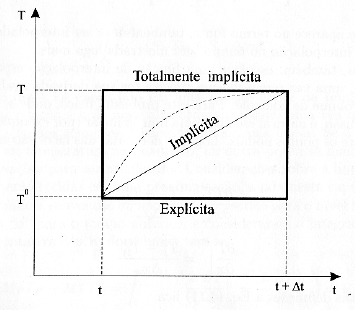
\includegraphics[width=8cm]{Imagenes/Funcion_Interpolacion.png}
\caption[Función de interpolación en el tiempo]{Función de interpolación en el tiempo. Modificado de Maliska(2006) \cite{Maliska2017TransferenciaEd..}}
\label{fig:fig34}
\end{figure}
%/////////////////////////////////////////////////////////////////////////////////////////


%........................................................................................
% TITULO DE LA SUBSECCIÓN 3.4.2.4
\subsubsection{Medio Poroso Saturado}~\hypertarget{sec:sec3424}{}
\label{sec:sec3424}




%........................................................................................
% TITULO DE LA SUBSECCIÓN 3.4.2.5
\subsubsection{Medio Poroso Parcialmente Saturado}~\hypertarget{sec:sec3425}{}
\label{sec:sec34245}




%----------------------------------------------------------------------------------------
% TITULO DE LA SECCIÓN 3.5
\section{Modelo Computacional}~\hypertarget{sec:sec350}{}
\label{sec:sec350}


%........................................................................................
% TITULO DE LA SUBSECCIÓN 3.5.1
\subsection{Consolidación Unidimensional}~\hypertarget{sec:sec351}{}
\label{sec:sec351}

%........................................................................................
% TITULO DE LA SUBSECCIÓN 3.5.1.1
\subsubsection{Realidad}~\hypertarget{sec:sec3511}{}
\label{sec:sec3511}


%........................................................................................
% TITULO DE LA SUBSECCIÓN 3.5.1.2
\subsubsection{Modelo Conceptual}~\hypertarget{sec:sec3512}{}
\label{sec:sec3512}


%........................................................................................
% TITULO DE LA SUBSECCIÓN 3.5.1.3
\subsubsection{Modelo Numérico}~\hypertarget{sec:sec3513}{}
\label{sec:sec3513}


%........................................................................................
% TITULO DE LA SUBSECCIÓN 3.5.1.4
\subsubsection{Modelo Computacional}~\hypertarget{sec:sec3514}{}
\label{sec:sec3514}


%........................................................................................
% TITULO DE LA SUBSECCIÓN 3.5.1.5
\subsubsection{Resultados de la Simulación}~\hypertarget{sec:sec3515}{}
\label{sec:sec3515}



%........................................................................................
% TITULO DE LA SUBSECCIÓN 3.5.1.6
\subsubsection{Validación}~\hypertarget{sec:sec3516}{}
\label{sec:sec3516}


%........................................................................................
% TITULO DE LA SUBSECCIÓN 3.5.2
\subsection{Consolidación Bidimensional}~\hypertarget{sec:sec352}{}
\label{sec:sec352}


%........................................................................................
% TITULO DE LA SUBSECCIÓN 3.5.2.1
\subsubsection{Realidad}~\hypertarget{sec:sec3521}{}
\label{sec:sec3521}


%........................................................................................
% TITULO DE LA SUBSECCIÓN 3.5.2.2
\subsubsection{Modelo Conceptual}~\hypertarget{sec:sec3522}{}
\label{sec:sec3522}



%........................................................................................
% TITULO DE LA SUBSECCIÓN 3.5.2.3
\subsubsection{Modelo Numérico}~\hypertarget{sec:sec3523}{}
\label{sec:sec3523}


%........................................................................................
% TITULO DE LA SUBSECCIÓN 3.5.1.4
\subsubsection{Modelo Computacional}~\hypertarget{sec:sec3524}{}
\label{sec:sec3524}


%........................................................................................
% TITULO DE LA SUBSECCION 3.5.1.5
\subsubsection{Resultados de la Simulación}~\hypertarget{sec:sec3525}{}
\label{sec:sec3525}


%........................................................................................
% TITULO DE LA SUBSECCIÓN 3.5.1.6
\subsubsection{Validación}~\hypertarget{sec:sec3526}{}
\label{sec:sec3526}



%........................................................................................
% TITULO DE LA SUBSECCIÓN 3.5.3
\subsection{Problema \textit{Five-Spot}}~\hypertarget{sec:sec353}{}
\label{sec:sec353}


%........................................................................................
% TITULO DE LA SUBSECCIÓN 3.5.4
\subsection{Verificación del Modelo Numérico}~\hypertarget{sec:sec354}{}
\label{sec:sec354}

